\documentclass[a4paper, 10pt]{memoir}


\usepackage[utf8]{inputenc} 
\usepackage{geometry}
\usepackage{amsmath, amsfonts, amssymb, amsthm, mathtools}
\usepackage{graphicx}
\usepackage{parskip}
\usepackage{fancyhdr}
\usepackage{lastpage}
\usepackage{optidef}
\usepackage{hyperref}
\usepackage{tikz}

\usepackage[
style=ieee]
{biblatex}
\addbibresource{sources.bib}


\chapterstyle{ger}
\maxsecnumdepth{subsection}
\maxtocdepth{subsection}

\pagestyle{fancy}
\fancyhf{}
\lhead{\rightmark}
\rhead{\leftmark}
\rfoot{Page \thepage \hspace{1pt} of \pageref{LastPage}}

\renewcommand{\headrulewidth}{1pt}
\renewcommand{\footrulewidth}{1pt}

\title{Specialization Project}
\author{Ulrik Bernhardt Danielsen}

\theoremstyle{plain}
\newtheorem{theorem}{Theorem}[section]
\newtheorem{lemma}{Lemma}[section]
\newtheorem{corollary}{Corollary}[theorem]
\newtheorem{proposition}{Proposition}[section]

\theoremstyle{definition}
\newtheorem{definition}{Definition}[section]
\newtheorem{example}{Example}[section]

\theoremstyle{remark}
\newtheorem*{remark}{Remark}


\newlength{\tpheight}\setlength{\tpheight}{0.9\textheight}
\newlength{\txtheight}\setlength{\txtheight}{0.9\tpheight}
\newlength{\tpwidth}\setlength{\tpwidth}{0.9\textwidth}
\newlength{\txtwidth}\setlength{\txtwidth}{0.9\tpwidth}
\newlength{\drop}


\newcommand*{\titleMS}{\begingroup% Thesis
\drop=0.1\txtheight
\vspace*{\drop}
\centering 
{\LARGE Norwegian Institute of Science and Technology}\\[2\baselineskip]
{\LARGE\sffamily Clustering animal behavior \par}
\vfill
{\LARGE TMA4500}\par
\vspace{\drop}
{\large Specialization project in Industrial Mathematics \\
        autumn 2022, supervised by Associate Professor  \\
        Benjamin Adric Dunn\par}
\vfill
{\large\bfseries Ulrik Bernhardt Danielsen}\par
\vspace*{\drop}
\endgroup}


\begin{document}

\begin{titlingpage}
\titleMS
\end{titlingpage}

\tableofcontents*
\clearpage
\listoffigures*
\clearpage

\lhead{}
\rhead{}
\begin{abstract}
        This specialization project serves as a preparation for the master thesis in Industrial Mathematics at NTNU. 
        My aim is to extend and justify a clustering methodology grouping motion recordings of free roaming rats into distinct behaviours.
        Using time frequency analysis to extract information about repeating movement patterns, and dimensionality reduction techniques such as principal component analysis and t-distributed stochastic neighbor embedding, we can separate behaviors in a two dimensional space.
        These detected behaviors can then be used further research, e.g., investigating connections between neural recordings and behavior, or behavioral effects by various stimulation.
\end{abstract}



\chapter{Introduction}
\lhead{\rightmark}
\rhead{\leftmark}
\section{Motivation}
The human brain is an incredibly complex structures that researchers have been trying to understand for a long time.
One way to gain information about how the brain operates is to study its neurons.
Neurons are cells which can communicate with each other through synapses.
This communication are electric signals and can be recorded.
At Kavli Institute for Systems Neuroscience at NTNU they are interested in relating these neural spike recordings to the behavior in rats.
This in turn begs the question of how rats behave.
Manually labelling video recordings of rats running around seems a tedious and unfruitful endeavor.
Additionally it introduces bias in our prior assumptions of how the rats behave, and which activities they engage in.
Thus, a methodology for automatically detecting distinct behaviours is needed.

\section{Previous work}
Through recent advances in machine learning and computer vision, many attempts at decomposing animal behavior into small modules has been made.
Manually labelling recordings of \textit{Drosophila melanogaster}, the fruit fly, before applying machine learning predation techniques shows performance on par with human labelling \cite{kain}
Unsupervised clustering techniques have also been developed for the fruit fly, using dimensionality reduction techniques to separate distinct behaviors in a two dimensional space \cite{berman}.
Research has not only been done on the fruit fly.
The MoSeq group at Harvard university uses 3D video capturing on free ranging mice.
Modelling the behavior modules as vector autoregressive processes, and changes between modules as a hidden Markov model, allows researches to extract information about rat body language and behavior \cite{wiltschko}.
Recording the behavior in 3D as opposed to 2D plays a big part of these methods success \cite{marshall}
As opposed to using depth cameras to provide the 3D kinematic recording, use of motion sensors have also been used. 





\chapter{Theory}
\section{Time series analysis}
We define time series as a realization $y_t = \{ y_{t_1}, y_{t_2}, \hdots, y_{t_n} \}$ of a stochastic process $Y(\omega, t)$, where $\omega \in \Omega$, $\Omega$ being the sample space,  and $t \in \mathbb{Z}$, $\mathbb{Z}$ being the chosen index set  \cite{wei}.
It is an ordered series of random variables which can be described completely by its joint probability function
\begin{equation*}
        F_{t_1,\hdots, t_n}(x_1, \hdots, x_n) = \text{Pr}\{ y_{t_1} \leq x_{1}, \hdots, y_{t_n} \leq x_n) \}.
\end{equation*}
The mean and variance function of a time series $y$ are defined as
\begin{equation}\label{eq:mean_func}
        \mu_t = E(y_t)  
\end{equation}
and
\begin{equation*}
        \sigma_t^2 = E(y_t - \mu_t)^2.
\end{equation*}

Given two random variables in the series $y_{t_1}$ and $y_{t_2}$, we define the covariance function and correlation function as
\begin{equation}\label{eq:acv}
        \gamma (t_{1}, t_2) = E[(y_{t_1} - \mu_{t_1})(y_{t_2} - \mu_{t_2})]
\end{equation}
and 
\begin{equation}\label{eq:acf}
        \rho(t_1, t_2) = \frac{\gamma ( t_1, t_2)}{\sqrt{\sigma_{t_1}^2}\sqrt{\sigma_{t_2}^{2}}}.
\end{equation}



\subsection{Stationarity}
A time series $y_t$ is $n$th-order stationary if for any shift $h$ and indexes $t_1, t_2, \hdots, t_n$ if 
\begin{equation}\label{eq:nth_stationary}
        F_{y_{t_1}, \hdots, y_{t_n}}(x_1, \hdots, x_n) = F_{y_{t_{1}+h}, \hdots, y_{t_{n} +h}} (x_1, \hdots, x_n).
\end{equation}
If \eqref{eq:nth_stationary} holds for all $n$, the time series is called \textit{strictly} stationary.
We also define a $n$th-order \textit{weakly} stationary time series $y_t$ if the first $n$ joint moments are finite and time invariant.
Specifically we define the second-order weakly stationary, i.e. with constant and time invariant mean function \eqref{eq:mean_func}, and where the covariance function \eqref{eq:acv} is solely a function of the time difference, as \textit{covariance} stationary.
When the covariance function between $t_1, t_2$ can be written as a function of the time difference $h = |t_1 - t_2|$, i.e. $\gamma (t_1, t_2) = \gamma (h) = \gamma_h$, we call it an \textit{autocovariance} function. 
The same is true for the correlation function \eqref{eq:acf}, which when is a function of the time difference is called an \textit{autocorrelation} function (ACF).
Figure \ref{fig:time_series_example} shows an example of a time series.
As the mean seem to increase with $t$ it is non-stationary.

\begin{figure}[tb]
        \centering
        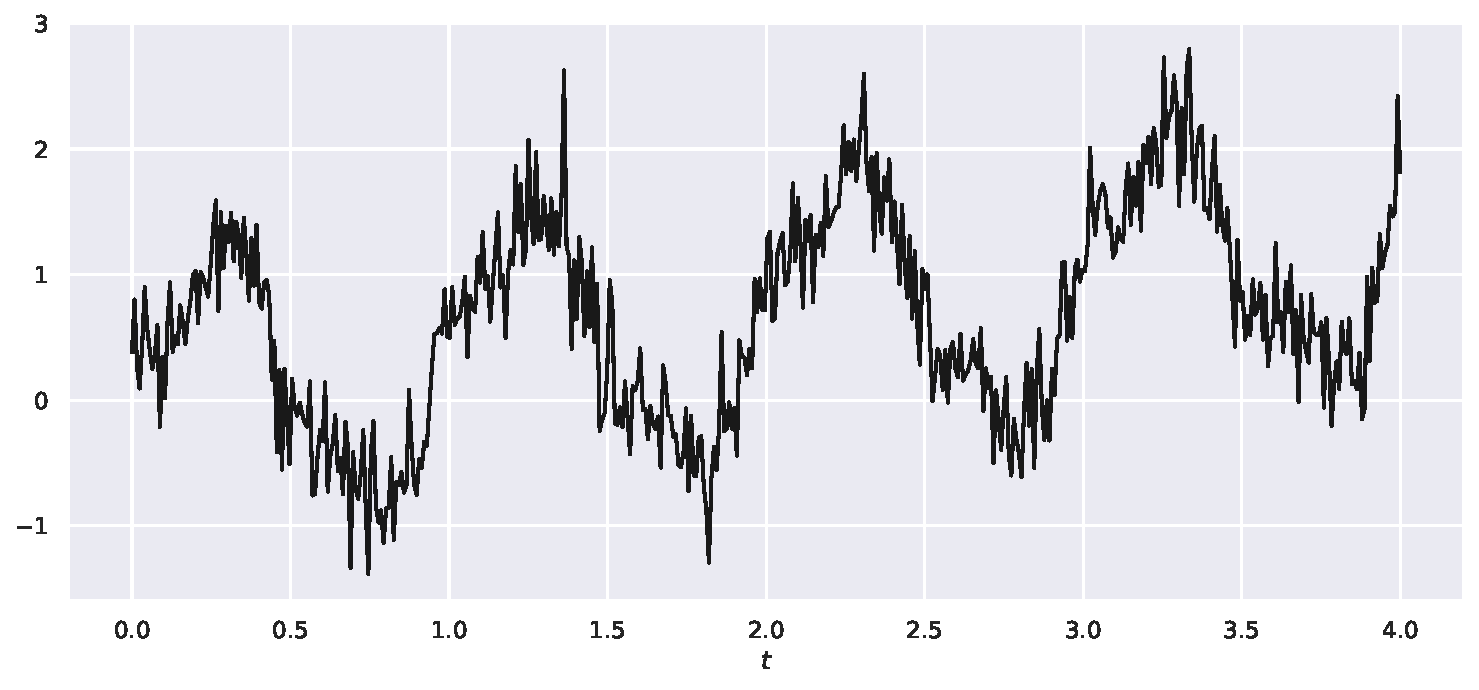
\includegraphics[width=\linewidth]{./code/figures/time_series_example.pdf}
        \caption{Example of a non-stationary time series with $t_0 = 0, t_n = 4$.
        The discrete data points are connected to better visualize the movement through time.}
        \label{fig:time_series_example}
\end{figure}

We also define the common estimates for the mean and covariance functions.
They are called the sample mean and sample covariance, and are written as
\begin{align}\label{eq:sample_mean}
        \bar{y_t} &= \frac{1}{n}\sum_{i = 1}^{n} y_{t_i}, \\
        \label{eq:sample_covariance}
        \hat{\gamma}_h &= \frac{1}{n} \sum_{i = 1}^{n - h}(y_{t_i} - \bar{y_t})(y_{t_i  + h} - \bar{y_t}),
\end{align}
respectively.


\subsection{Detrending}
Many methods for analysing and processing time series requires stationarity \cite{shumway}.
If the series is non-stationary, we can split the it into one stationary and one non-stationary part called the \textit{trend}.
Mathematically we write it as 
\begin{equation*}
        y_t = \mu_t + x_t,
\end{equation*}
where $x_t$ denotes the stationary part and $\mu_t$ the trend.
The process of finding $\mu_t$ and then computing $x_t = y_t - \mu_t$ is called \textit{detrending}.
Detecting the trend can be done in many ways, for instance using regression techniques or smoothing.
The simplest way is to assume a linear trend, $\mu_t = \beta_0 + \beta_1 t$ and estimate the parameters using least squares.
In figure \ref{fig:time_series_example_with_trend} the linear regression fit is shown, showing an upwards in the time series.


\begin{figure}[tb]
        \centering
        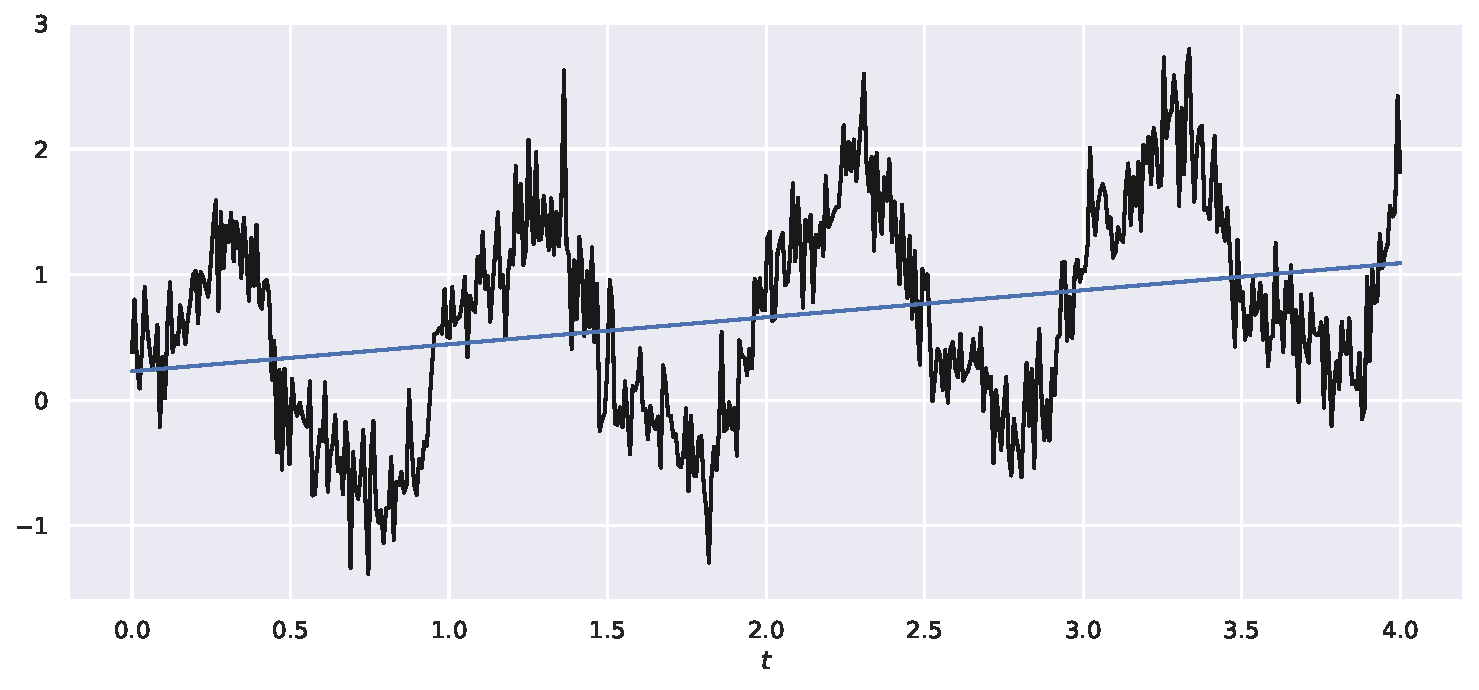
\includegraphics[width=\linewidth]{./code/figures/time_series_example_with_trend.pdf}
        \caption{Time series from figure \ref{fig:time_series_example} with an estimated linear trend shown in blue.}
        It is clear that there exists an upward trend in the data.
        \label{fig:time_series_example_with_trend}
\end{figure}




\section{Fourier analysis}
Let $Z_1, Z_2, \hdots, Z_n$ be a sequence of numbers.
For simplicity in notation we assume $n$ to be an odd number.
It can be shown that the sequence can be represented as a linear combination of complex exponentials
\begin{equation}\label{eq:fourier_series}
        Z_t = \sum_{k = -\frac{n-1}{2}}^{\frac{n- 1}{2}}c_k e^{\frac{i2 \pi k t}{n}}.
\end{equation}
This comes from the fact that the set 
\begin{equation*}
        \left\{ e^{\frac{i 2 \pi kt}{n}} \Big| k \in \left[ -\frac{n -1}{2}, \frac{n - 1}{2} \right] \right\}
\end{equation*}
consists of $n$ orthogonal functions \cite{wei}.
I.e., that
\begin{equation*}
        \sum_{i = 1}^{n} e^{\frac{i2 \pi kt}{n}} e^{-\frac{i 2 \pi j t}{n}}= 
                \begin{cases}
                        n, & k = j \\
                        0, & k \neq j \\
                \end{cases}
       .
\end{equation*}
The coefficients $c_k$ are given by
\begin{equation*}
       c_k =  \frac{1}{n}\sum_{ t = 1}^{n}Z_t e^{-\frac{i 2\pi kt}{n}}.
\end{equation*}
It is clear that \eqref{eq:fourier_series} is periodic with period $n$, meaning $Z_{t + jn} = Z_t, j = 0, \pm 1, \pm 2, \hdots$.
Thus the Fourier series is able to capture periodic sequences.
The smallest positive integer $n$ for which $Z_{t + n} = Z_t$ is called the fundamental period, with corresponding fundamental frequency $2 \pi /n$.
For the components $k = \pm j, j = 1, 2, \hdots, (n-1)/2$ the frequencies are multiples of the fundamental frequency, $\omega_k = k(2\pi/n)$.
The set of frequencies making up the series is called the \textit{spectrum}.
As a consequence the coefficients $c_k$ can be viewed as weighting the importance of the contributions for the different frequencies making up the full sequence.
This is formalized by the definitions of energy and power,
\begin{align}\label{eq:energy}
        &\text{energy} = \sum_{t = 2}^{n} Z_t^2 = n \sum_{k = -\frac{n -1}{2}}^{\frac{n - 1}{2}} |c_k|^2 ,\\ 
        \label{eq:power}
        &\text{power} = \frac{\text{energy}}{n} = \sum_{k = -\frac{n -1}{2}}^{\frac{n - 1}{2}} |c_k|^2. 
\end{align}
Let $p_k$ be the contribution to the power from frequency $k = 0, 1, \hdots, (n-1)/2$.
As $\omega_k$ and $\omega_{-k}$ corresponds to the same frequency the contribution is given as $p_0 = c_0^2, p_k = 2|c_k|^2, k = 1, \hdots, (n-1)/2$.
The values $p_k$ are called the power spectrum of the series.


\subsection{Discrete-Time Fourier Transform}
We have seen that all sequences of length $n$ can be viewed and parameterized as Fourier series with period $n$.
Moving to non-periodic sequences essentially amounts to taking the limit of the series as $n$ approaches infinity.
Formally we now let $Z_t$ be a finite discrete function of $t$, where $Z_t = 0$ when $|t| > M$ for some integer $M$.
Choosing $n = 2M + 1$ the function
\begin{equation*}
        Y_{t + jn} = Z_t, \ t \in \left[ -\frac{n-1}{2}, \frac{n-1}{2} \right], \ j \in \mathbb{Z}
\end{equation*}
is periodic with period $n$.
It's Fourier series is 
\begin{equation*}
        Y_t = \sum_{k = -\frac{n - 1}{2}}^{\frac{n -1 }{2}} c_k e^{\frac{i2 \pi kt}{n}}.
\end{equation*}
As $Y_t = Z_t$ when $t \in [-(n-1)/2, (n-1)/2]$, and $Z_t = 0$ when $|t| > (n-1)/2$, the coefficients $c_k$ can be written as the infinite sum
\begin{align*}
        c_k &= \frac{1}{n}\sum_{t = - \infty}^{\infty} Z_t e^{\frac{-i2\pi kt}{n}} \\
        & = \frac{2 \pi}{n}f\left(\frac{2\pi k}{n}\right),
\end{align*}
where 
\begin{equation*}
        f(\omega) = \frac{1}{2\pi} \sum_{t = -\infty}^{\infty} Z_t e^{-i\omega t}.
\end{equation*}
If we now take the limit $Z_t = \lim_{n \rightarrow \infty} Y_t$ the summation becomes an integral over the length $2\pi$ \cite{wei}.
This gives the relation
\begin{align}\label{eq:dtft_inv}
        Z_t &= \int_{-\pi}^{\pi} f(\omega) e^{i\omega t} d\omega, \quad t \in \mathbb{Z} \\
        \label{eq:dtft}
        f(\omega) &= \frac{1}{2 \pi} \sum_{t = -\infty}^{\infty} Z_t e^{-i \omega t}, \quad -\pi \leq \omega \leq \pi,
\end{align}
where $f(\omega)$ in \eqref{eq:dtft} is called the discrete-time Fourier transform of $Z_t$.
As opposed to the periodic case \eqref{eq:fourier_series} where the periodic sequence was made up by a finite number of frequencies, the non-periodic sequence is an integral over a continuum of frequencies $\omega$.
We call $|f(\omega)|$ the spectrum of the sequence, and the function $g(\omega) = 2 \pi |f(\omega)|^2$ the energy spectrum.
The energy spectrum definition comes from Parseval's relation 
\begin{equation}\label{eq:parseval}
        \sum_{t = -\infty}^{\infty} |Z_t|^2 = 2 \pi \int_{- \pi}^{\pi}|f(\omega)|^2 d\omega.
\end{equation}
It is worth noting that the relation in \eqref{eq:parseval} only holds when the sequence $Z_t$ is absolutely summable, i.e., that
\begin{equation}\label{eq:absuletly_summable}
        \sum_{ t = -\infty}^{\infty}|Z_t| < \infty.
\end{equation}

\section{Spectral density estimation}
Let $y_t$ be a stationary time series where the autocovariance function $\gamma_h$ from \eqref{eq:acv} is absolutely summable.
Then we can write $\gamma_h$ as a Fourier transform pair
\begin{align}\label{eq:spectrum}
        f(\omega) &= \frac{1}{2 \pi} \sum_{h = -\infty}^{\infty} \gamma_h e^{-i\omega h}, \\
        \label{eq:spectral_dens_inv}
        \gamma_h &= \int_{-\pi}^{\pi} f(\omega)e^{i\omega h}d\omega.
\end{align}
It can be shown \cite{shumway} that the spectrum $f(\omega)$ in \eqref{eq:spectrum} is real-valued and non-negative.
Furthermore, as $\text{Var}(y_t) = \gamma_0$, we get the interpretation
\begin{equation*}
        \text{Var}(y_t) = \int_{-\pi}^{\pi}f(\omega)d\omega,
\end{equation*}
i.e., that $f(\omega)$ is the contribution to the variance for frequency $\omega$.
We often want to locate these important frequencies,  and thus an important task is to estimate this spectrum.

\subsection{Periodogram}
Again we consider a time series sample $y_1, y_2, \hdots, y_n$ where $n$ is chosen to be odd for simplicity.
It can be written as a real Fourier representation 
\begin{equation*}
        y_t = a_0 + \sum_{k = 1}^{\frac{n-1}{2}} (a_k \cos(\omega_k t) + b_k \sin (\omega_kt)),
\end{equation*}
where $\omega_k = 2\pi k / n, k =0, 1, \hdots, (n -1)/2$ and the coefficients are given as 
\begin{equation*}
        a_0 = \bar{y_t}, \quad a_k = \frac{2}{n}\sum_{t = 1}^{n}y_t \cos(\omega_kt), \quad b_k = \frac{2}{n} \sum_{ t = 1}^{n} y_t \sin (\omega_kt).
\end{equation*}
We then define the periodogram as 
\begin{equation}\label{eq:periodogram}
        I(\omega_k) = 
                \begin{cases}
                        na_0^2, & k=0  \\
                        \frac{n}{2}(a_k^2 + b_k^2), & k = 1, \hdots, (n-1)/2. \\
                \end{cases}
\end{equation}
The periodogram is of interest as it has has a large value if the frequency $\omega_k$ is of importance in the series.
A scaled periodogram $\frac{2}{n}I(\omega_k)$ estimates the sample variance of the sinusoid component at frequency $\omega_k$ \cite{shumway}.
A periodogram for the time series example in figure \ref{fig:time_series_example} are shown in figure \ref{fig:periodogram_basic}.
Note that the time series is linearly detrended for the periodogram is computed.
The two highest peaks match the underlying generating function which can be revealed to be $\sin(2\pi t) + \frac{1}{4} \cos(6 \pi t) + t / 3$.

\begin{figure}[tb]
        \centering
        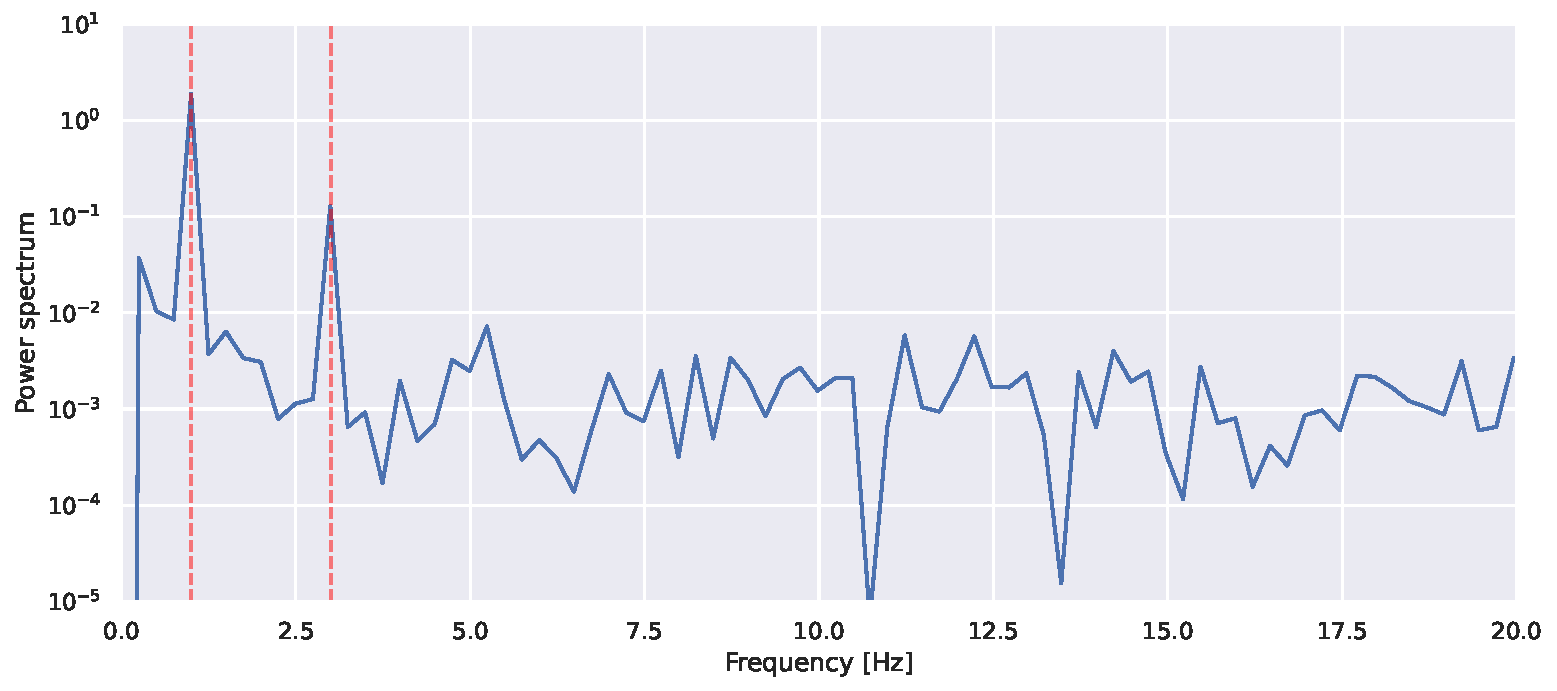
\includegraphics[width=\linewidth]{./code/figures/periodogram_basic.pdf}
        \caption{Periodogram for the time series plotted in figure \ref{fig:time_series_example}.
        The time series is detrended assuming a linear trend.
        Observe that the two highest peaks in the periodogram are at the underlying frequencies $1$Hz and $3$Hz shown with dashed red lines.}
        \label{fig:periodogram_basic}
\end{figure}




\subsection{Sample spectrum}
One intuitive way of estimating the spectrum is to replace the autocovariance with the sample autocovariance from equation \eqref{eq:sample_covariance}.
I.e., we define the sample spectrum for a realization $y_1, y_2,  \hdots, y_n$
\begin{equation}\label{eq:sample_spectrum}
        \hat{f}(\omega) = \frac{1}{2\pi}\sum_{k = -(n - 1)}^{n-1}\hat{\gamma}_k e^{-i\omega k}.
\end{equation}
At the Fourier frequencies $\omega_k$ it is related to the periodogram through \cite{wei}
\begin{equation*}
        \hat{f}(\omega_k) = \frac{I(\omega_k)}{4 \pi}.
\end{equation*}
Although $\hat{f}(\omega_k)$ is asymptotically unbiased, meaning $\lim_{n \rightarrow \infty} E(\hat{f}(\omega)) = f(\omega)$, is lacks consistency in the variance as $n$ tends to infinity, i.e.,
\begin{equation*}
        \lim_{n \rightarrow \infty} \text{Var}(\hat{f}(\omega_k)) \neq 0.
\end{equation*}


\subsection{Spectral Window}
The fact that the variance does not decrease with the sample size produces quite jagged and noisy spectrum estimations \cite{shumway}.
To account for this we introduce the spectral window which smooths the spectrum.
Mathematically the smoothed spectrum is written as
\begin{equation}\label{eq:smo_spec}
        \hat{f}_{\mathcal{W}}(\omega_k) = \sum_{j = -m}^{m} \mathcal{W}_n(\omega_j) \hat{f}(\omega_k - \omega_j),
\end{equation}
where $\omega_k = 2\pi k/n,\ k = 0,1, \hdots, (n-1)/2$ and $m$ is a function of $n$, typically $m \ll n$.
The value of $m$ decides how many points in the neighborhood of $\omega_k$ should be included in the smoothing.
Furthermore, the function $\mathcal{W}_n(\omega_j)$ is chosen to have the following properties,
\begin{align}
        &\sum_{j = -m}^{m}\mathcal{W}_n(\omega_j) = 1, \nonumber \\
        &\mathcal{W}_n(\omega_j) = \mathcal{W}_n(-\omega_j), \nonumber \\
        \label{eq:w_var}
        &\lim_{n \rightarrow \infty} \sum_{j = -m}^{m}\mathcal{W}_n^2(\omega_j) = 0.
\end{align}
We view the smoothed spectrum as a weighted average of the sample spectrum \eqref{eq:sample_spectrum} in a window around the target frequency $\omega_k$.
How the weights are distributed in the window is governed by $\mathcal{W}_n(\omega_j)$, giving it the name spectral window.
Because of the property in \eqref{eq:w_var} we have
\begin{align*}
        \text{Var}(\hat{f}_\mathcal{W}(\omega_k)) &\approx \sum_{j = -m}^{m}\mathcal{W}_n^2(\omega_j)(f(\omega_k))^2 \\
                                             &=(f(\omega_k))^2 \sum_{j = -m}^{m} \mathcal{W}_n^2(\omega_j) \overset{n \rightarrow \infty}{=} 0,
\end{align*}
assuming $f(\omega)$ is approximately constant in the window.
We can thus reduce the variance by increasing the points included in the window.
However, when doing so we introduce bias.


\subsection{Lag window}
It can be shown \cite{wei} that the spectral window forms a Fourier transform pair with a lag window $W_n(k)$, i.e,
\begin{equation*}
        W_n(k) = \int_{-\pi}^{\pi}\mathcal{W}_n(\omega) e^{i\omega k}d\omega, \quad k = 0, \pm 1, \hdots, \pm M.
\end{equation*}
The lag window is a weighting function applied to the sample autocovariance 
\begin{equation*}
        \hat{f}_\mathcal{W} = \frac{1}{2\pi} \sum_{k = -M}^{M}W_n(k) \hat{\gamma}_k e^{-i\omega k},
\end{equation*}
with $W_n = W(k/M)$, $W$ being a bounded even continuous function 
\begin{align*}
        &|W(t)| \leq 1, \\
        &W(0) =, \\
        &W(t) = W(-t), \\
        &W(t) = , \  t > 1.
\end{align*}
Figure \ref{fig:windows} shows the popular \textit{hanning} window given by 
\begin{equation}\label{eq:hann}
        W_n^H=
                \begin{cases}
                      \frac{1}{2}(1 + \cos(\frac{\pi k}{M})),   & |k| \leq M \\
                       0,  & |k| > M, \\
                \end{cases}
\end{equation}
with $M = 5$.


\begin{figure}[tb ]
        \centering
        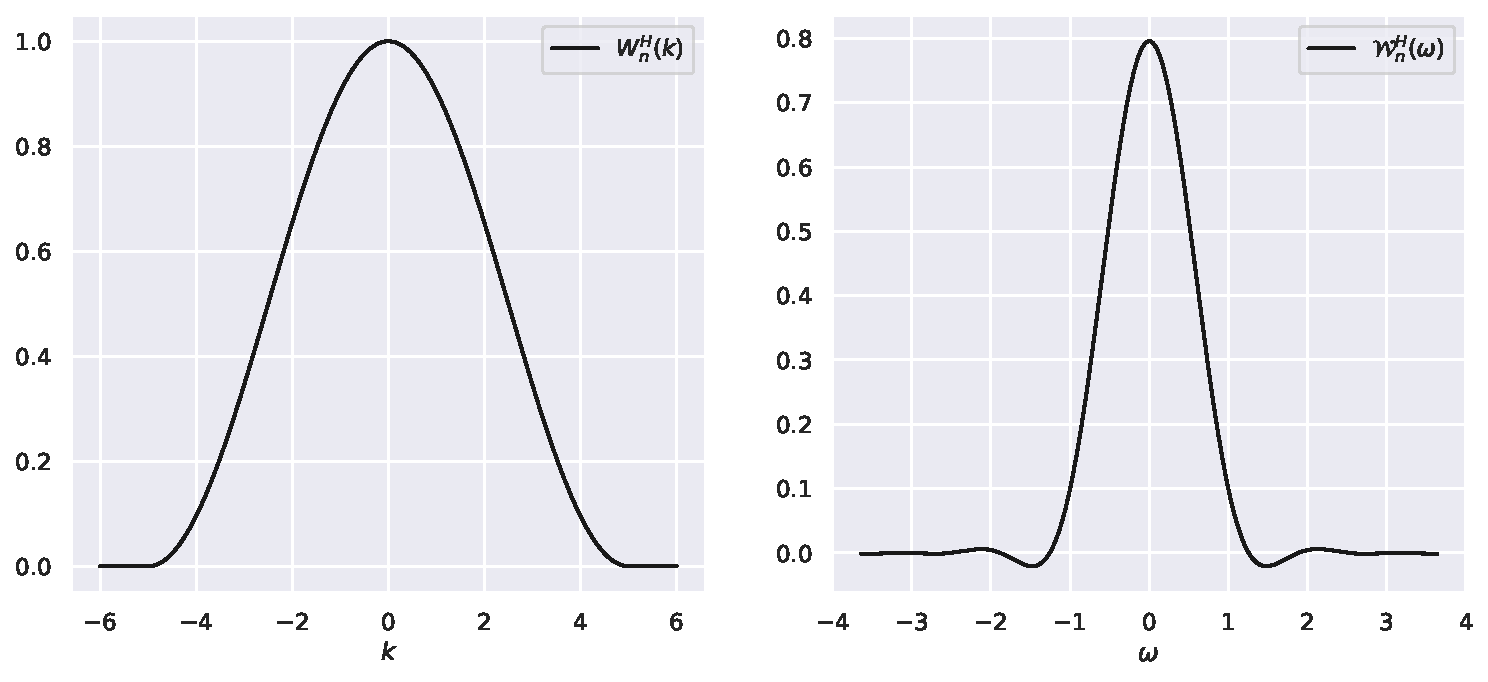
\includegraphics[width=\linewidth]{./code/figures/windows.pdf}
        \caption{On the left the hanning window given by equation \eqref{eq:hann}.
        On the left the corresponding spectral window, i.e., its Fourier transform.}
        \label{fig:windows}
\end{figure}



\section{Time frequency analysis}
The methods mentioned so far are only suitable for extracting information about the frequencies of a signal.
If the process is stationary this is often all we need.
However, if the process is non-stationary and the frequencies change over time, the periodogram is unable to capture this.
The original time series contains all the information in the time-scale, and the Fourier transform contains all the information in the frequency scale.
We need something in between.

\subsection{Short-Time Fourier Transform}
A simple and intuitive way to gain information about the changes in frequency is to divide the time interval into sections, and compute the Fourier transform on each section.
Then we can plot how the periodogram changes over time.
If we divide the time interval using a window function this method is called the short-time Fourier Transform (STFT).
Mathematically we define it for a discrete sequence $y = y_1, y_2, \hdots, y_n$, which is windowed by $W_n(t)$ around time $\tau$, as
\begin{equation}\label{eq:stft}
        S_y(\omega, \tau) = \frac{1}{2 \pi} \sum_{t = -\infty}^{\infty}y_t W_n(t - \tau)e^{-i\omega t}.
\end{equation}
The estimated spectrum $|S_y(\omega, \tau)|^2$ is now a function of both time and frequency, and is commonly called the spectrogram \cite{cohen}, which can be plotted to show the changes in frequencies over time.

Unfortunately the STFT has some severe drawbacks; it can be shown that there exists a limit for the possible precision achieved when measuring both frequency and time simultaneously \cite{kaiser}.
There exists a tradeoff in time and frequency resolution, as shown in figure \ref{fig:grid}.
\begin{figure}[tb]
        \centering
        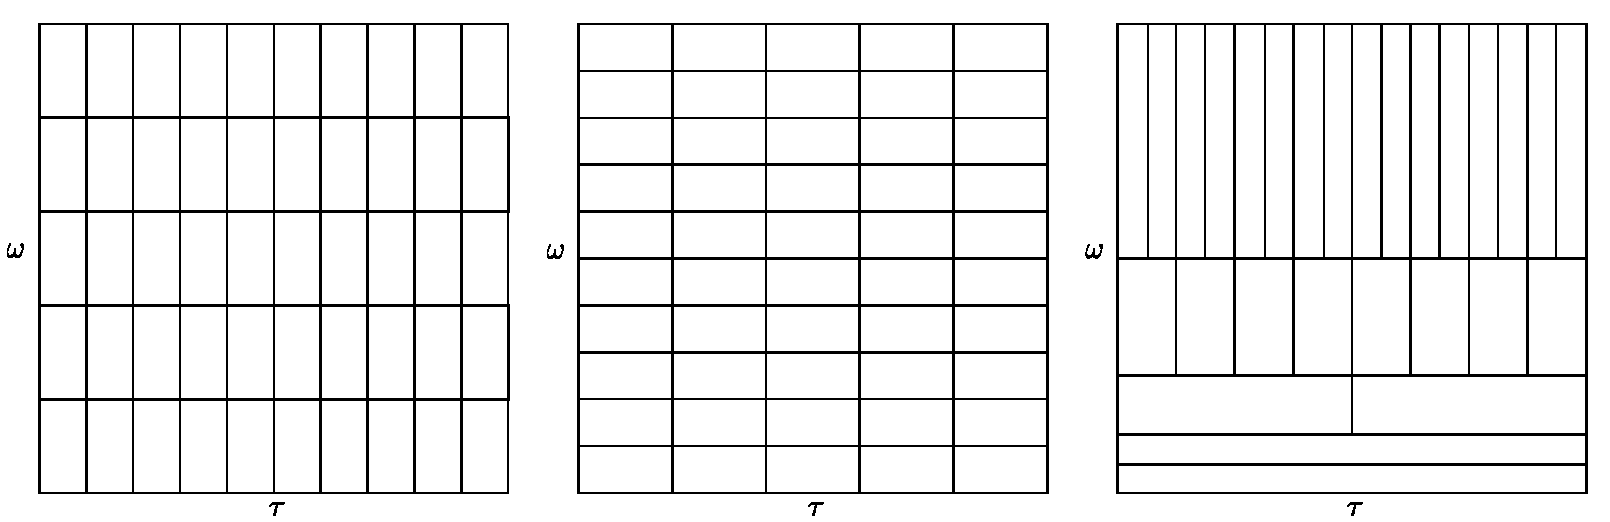
\includegraphics[width=\linewidth]{./figures/stft_cwt_grid/stft_cwt_grid.pdf}
        \caption{
        \textit{Left/middle:} The figures illustrates the tradeoff in resolution for time and frequency for the short-time Fourier transform from equation \eqref{eq:stft}, increasing the resolution in time decreases the resolution in frequency and vice versa.
\textit{Right:} Illustrate the corresponding resolution for the continuous wavelet transform from equation \eqref{eq:cwt}.
}
        \label{fig:grid}
\end{figure}
This is very intuitive as frequency has to be measured over a certain time period.
Decreasing the width of the window function makes detecting smaller frequencies harder, and vice versa.
Thus we need to know the approximate frequency scales in the data before performing the STFT, or we can try several window widths.
In the case where frequencies exists in the data on several different scales, the STFT in equation \eqref{eq:stft} becomes unsuitable.



\subsection{Wavelet transform}
The wavelet transform works in a very similar way as the STFT, but circumvents the problem of choosing a fixed width of the window by introducing scaling.
Let $\psi(t)$ be a window function (possibly complex valued) which we will call the mother wavelet.
One way of scaling the mother wavelet by a factor $s$ is
\begin{equation*}
        \psi_s(t) = \frac{1}{s^{1/2}} \psi \left(\frac{t}{s}\right).
\end{equation*}
If we also allow a time shift around $\tau$ we arrive at the wavelets
\begin{equation*}
        \psi_{s,\tau}(t) = \frac{1}{s^{1/2}} \left( \frac{t - \tau}{s} \right).
\end{equation*}
This culminates in the definition of the continuous wavelet transform (CWT) of a function $f$ \cite{kaiser}
\begin{equation}\label{eq:cwt}
        \tilde{f}(s, \tau)\int_{-\infty}^{\infty}\psi_{s,\tau}^*(t)f(t) dt,
\end{equation}
where $\psi_{s,\tau}^*$ is the complex conjugate of the function $\psi_{s, \tau}$.

Again considering the discrete sample $y_1, y_2, \hdots, y_n$ with $\delta t = y_{t+1} - y_t, \ t = 1, \hdots, n$, its continuous wavelet transform is given by \cite{torrence}
\begin{equation}\label{eq:cwt_d}
        \tilde{f}_n(s, \tau) = \sum_{t = 1}^{n} y_t \psi^* \left( \frac{\delta t}{s}(t- \tau) \right),
\end{equation}
where $\tau$ now is a time index $\tau \in \{ 1, 2, \hdots, n \}$.
It is computationally efficient \cite{torrence} to represent the CWT as the inverse Fourier transform
\begin{align*}
        &\tilde{f}_n(s, \tau) \sum_{t = 1}^{n}\hat{y}_k \hat{\psi}^*(s\omega_k)e^{i \omega_k n\delta t}, \\
        & \hat{y}_k = \frac{1}{n}\sum_{t = 1}^{n}y_t e^{-\frac{i2\pi kt}{n}},\\
        &\omega_k = 
                \begin{cases}
                      \frac{2\pi k}{n \delta t},   &  k \leq \frac{n}{2} \\
                      -\frac{2\pi k}{n \delta t},   &  k > \frac{n}{2} \\
                \end{cases}.
\end{align*}
As always we are interested in the power spectrum, which for the CWT is defined as $|\tilde{f}_n(s,\tau)|^2$.

There exists many choices for the mother wavelet, and certain important criteria it must satisfy \cite{kaiser}.
One popular wavelet is the Morlet wavelet defined as
\begin{equation}\label{eq:morlet}
        \psi_0(\eta) = \pi^{-1/4} e^{i\omega_0 \eta}e^{-\eta^2 / 2},
\end{equation}
where $\omega_0$ is a parameter chosen to fit the criteria.

In figure \ref{fig:scaleogram_ex} a scaleogram is shown for the function
\begin{equation}\label{eq:ex_scale}
        f(t) = 
                \begin{cases}
                        3 \sin(2.4 \cdot 2\pi t) + 2 \sin(4.7 \cdot 2 \pi t) + \sin(17 \cdot 2 \pi t), & t < 30 \\
                        \sin(0.7 \cdot 2 \pi t) + 2 \sin(1.4 \cdot 2 \pi t) + 3 \sin(6.4 \cdot 2 \pi t), & t \geq 30, \\
                \end{cases}
\end{equation}
with added Gaussian noise.
The continuous wavelet transform is computed at 18 frequencies between $0.5$Hz and $20$ Hz.

\begin{figure}[tb]
        \centering
        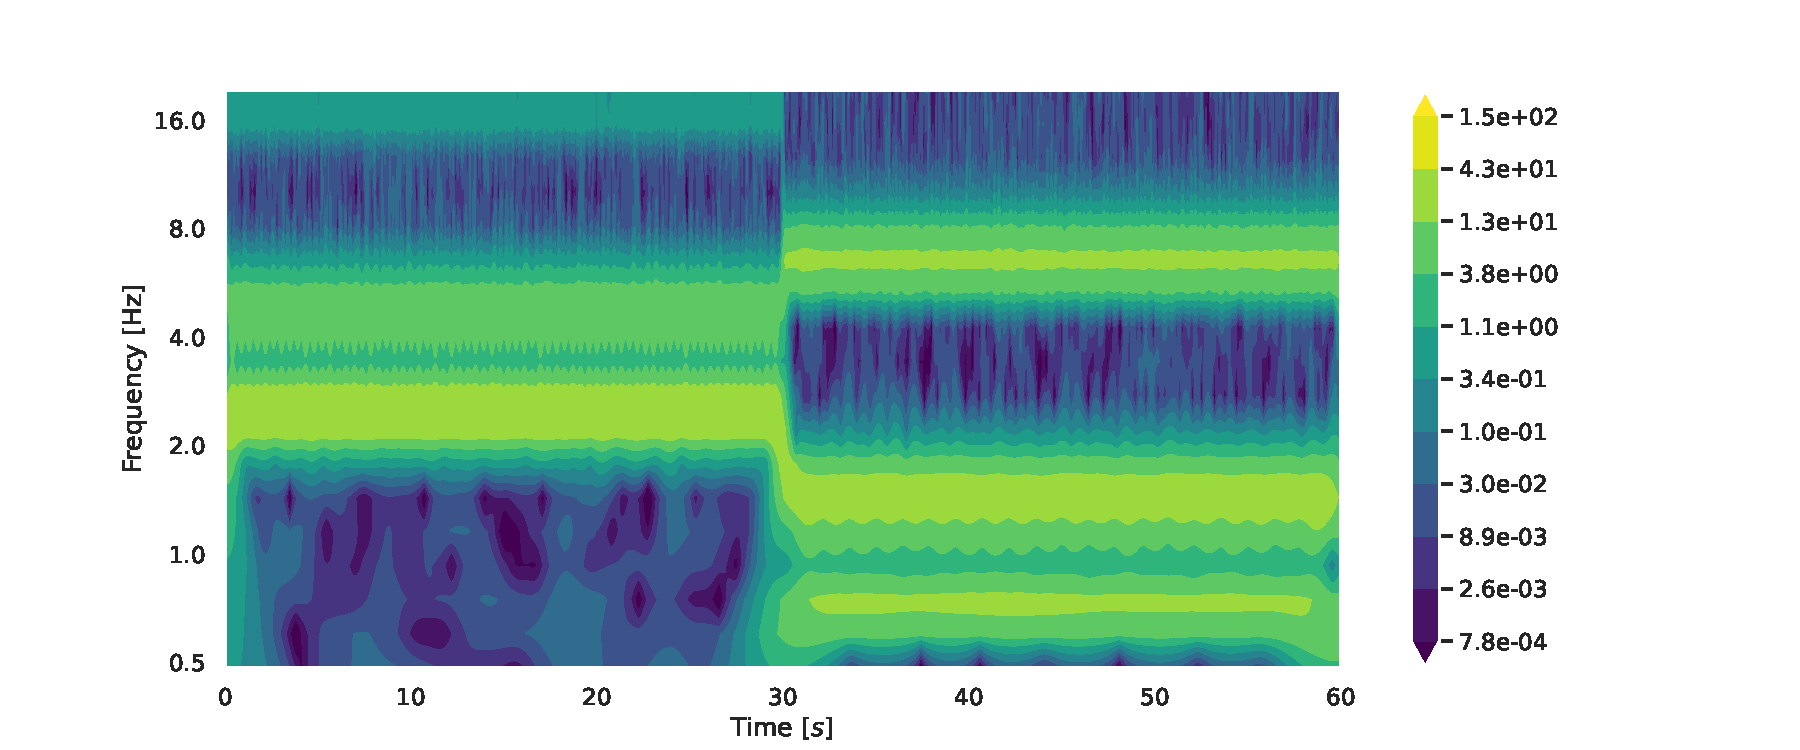
\includegraphics[width=\linewidth]{./code/figures/scaleogram_example.pdf}
        \caption{An example of a scaleogram of the continuous wavelet transform of function \eqref{eq:ex_scale} with added Gaussian noise.}
        \label{fig:scaleogram_ex}
\end{figure}



\section{Piecewise polynomials}
Suppose we have an interval $[a,b]$ divided into $M$ contiguous subintervals.
The connecting edges of the subintervals $a = \xi_0, \xi_1, \hdots, \xi_{M - 1}, \xi_{M} = b$ are called knots.
On each of the intervals $[\xi_i, \xi_{i+1}], i = 0, \hdots, M-1$ we define a polynomial $p_i (t)$.
The function
\begin{equation*}
        f(t) = 
                \begin{cases}
                        p_0(t), &  t \in [\xi_0, \xi_{1}) \\
                        p_1(t), & t \in [\xi_1, \xi_2)  \\
                        & \vdots \\
                        p_{M-1}(t), & t \in [\xi_{M-1}, \xi_{M}]  \\
                \end{cases}
\end{equation*}
is called a \textit{piecewise polynomial}.


\subsection{Splines}
In the definition of piecewise polynomials no restrictions are made on the polynomials, they are allowed to take any form.
As in \cite{quarteroni} we define a \textit{spline} $s_k(t)$ of order $k$ on the interval $[a,b]$ as a piecewise polynomial where
\begin{align*}
        &s_k(t) \in \mathcal{P}^k , \quad t \in [\xi_i, \xi_{i+1}],\quad i = 0, 1, \hdots, M-1 \\
        &s_k(t) \in \mathcal{C}^{k - 1}[a, b].
\end{align*}
I.e., the spline consists of piecewise polynomials of order $k$ and has continuous derivatives up to order $k - 1$.
A common choice is letting $k = 3$, providing continuous second derivatives over the interval.
This is called \textit{cubic} splines, and are often considered sufficiently smooth for function approximations.
It is also common to add curvature constraints at the endpoints, $s_3''(a) = s_3''(b)$, arriving at the \textit{natural} cubic splines.

\subsection{Regression splines}
Suppose now we have data points $y_{t_1}, y_{t_2}, \hdots, y_{t_n}$ on $[a = t_1, b = t_n]$. 
A spline of order $k$ with chosen knots at $a = t_1 = \xi_0, \xi_1, \hdots, \xi_{M} = t_n = b$ can be parameterized as 
\begin{equation}\label{eq:lsq_spline}
        s_k(t) = \sum_{i = 1}^{M + k} \beta_i h_i(t),
\end{equation}
where the functions $h_i$ are the truncated-power basis set
\begin{align*}
        h_j(t) &= t^{j - 1}, \ j = 1, \hdots, k+1, \\
        h_{k+1+l}(t) &= (t - \xi_l)_+^k, \ l = 1, \hdots, M-1,
\end{align*}
with $(t)_+ = \max_{} \{ t, 0 \}$ \cite{hastie}.
The parameters $\beta_i$ can be found using least squares.
An example of cubic spline regression are shown in figure \ref{fig:cubic_splines}.

\begin{figure}[tb]
        \centering
        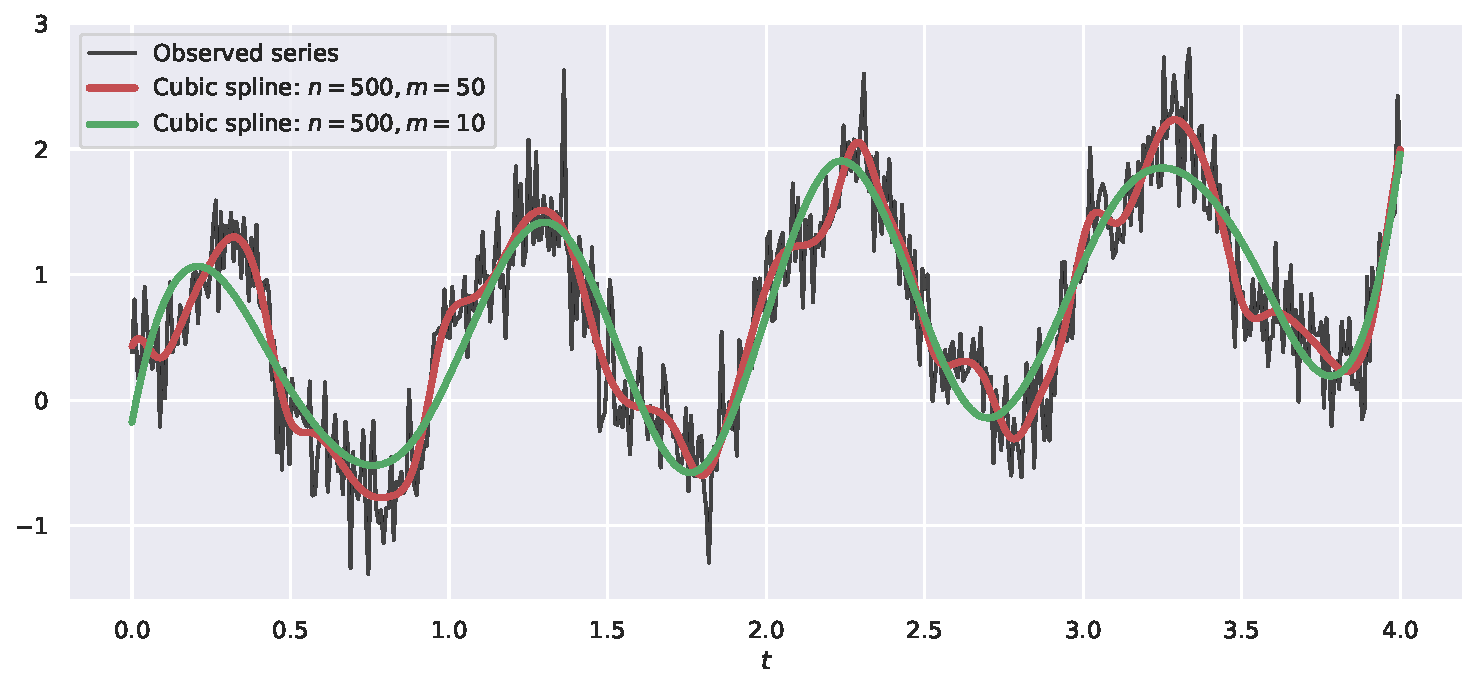
\includegraphics[width=\linewidth]{./code/figures/cubic_splines.pdf}
        \caption{Two cubic splines fitted using least square regression on the time series from figure \ref{fig:time_series_example}.
        Observe that the red spline with 50 knots (including endpoints) fits the data closer than the green spline with 10 knots.}
        \label{fig:cubic_splines}
\end{figure}




\section{Dimensionality reduction}
Suppose we have $n$ datapoints, each having $p$ numerical features. 
Mathematically we represent them as the vectors $x_i = (x_{i1}, x_{i2}, \hdots, x_{in} ) \in \mathbb{R}^p, \ i = 1, 2, \hdots, n$, often represented in the $n \times p$ data matrix $X, \ X_{ij} = x_{ij}, \ i = 1, 2, \hdots, n, \ j = 1, 2, \hdots, p$.
Dimensionality reduction is about finding a low dimensional representation of the data still containing most of its properties.
There can be many reasons for performing dimensionality reduction, and often it is performed as a form of feature extraction used before predictive modelling or clustering \cite{hastie}.
If the data is sparse or the features highly correlated, reducing the dimensionality could improve computation speed and remove noise.
Reducing the data to two dimensions often allows for easier visualization and interpretability of the data.



\subsection{Principal component analysis}\label{sec:pca}
One of the most commonly used dimensionality reduction methods is called principal component analysis (PCA).
There are multiple ways to both derive and interpret the method.
Given the $n \times p$ data matrix $X$ we find a sequence of $q \leq p$ orthogonal $p \times 1$ unit vectors $v_1, v_2, \hdots, v_q$, each one chosen such that $Z_j = Xv_j$ has maximum variance.
On matrix form we write it as $Z = X V_q$, where the columns of $V_q$ are $v_j, j = 1, 2, \hdots, q$. 
The principal components scores—which represents our new features when applying dimensionality reduction—is given by the $q$ columns in $Z$.
Let $S$ be the sample covariance matrix of $X$.
It can be shown \cite{jolliffe} that the vectors $v_j$ that maximises the variance while subject to the mentioned constraints, are the eigenvectors of $S$, with the corresponding eigenvalue $\lambda_j$. Note that $\lambda_i > \lambda_{i+1},\ i = 1, 2, \hdots, p-1$.
For this reason we need to standardize the columns of $X$ to have mean zero and variance one before applying PCA.
The proportion of the total variance explained by the first $q$ principal components is given by
\begin{equation*}
        \frac{\sum_{i = 1}^{q}\lambda_i}{\sum_{j = 1}^{p} \lambda_j}.
\end{equation*}
Thus when using PCA for dimensionality reduction we set a variance threshold, and keep the number of principal components keeping enough variance.



\subsection{t-Stochastic Neighbor Embedding}\label{sec:tsne}
Another dimensionality reduction method specially suited for visualizing data in two dimension, is called t-Stochastic Neighbor Embedding (t-SNE).
Again we start with the $n \times p$ data matrix, and wish to embed it into a low dimensional space preserving as much of the original structure in the data as possible.
Instead of trying to emulate the Euclidian distances between the data points $x_1, x_2, \hdots, x_n$, we convert them into conditional probabilities 
\begin{equation}\label{eq:gaus}
       p_{j|i} = \frac{\exp \left\{ \frac{-||x_i - x_j||^2}{2\sigma_i} \right\}}{\sum_{k \neq i}^{} \exp \left\{ \frac{-||x_i - x_k||^2}{2\sigma_i^2} \right\}}, \quad i \neq j, \ p_{i|i} = 0. 
\end{equation}
For a point $x_i$, $p_{j|i}$ is large for nearby points $x_j$, the magnitude proportional to a Gaussian distribution centered at $x_i$ with variance $\sigma_i^2$ \cite{hinton}.
The individual variance $\sigma_i^2$ is a tuning parameter to be chosen by the user.

In the low dimensional representation we model the similarities as joint probabilities based on the Student t-distribution with one degree of freedom
\begin{equation}\label{eq:student}
        q_{ij} = \frac{(1 + ||y_i - y_j||^2)^{-1}}{\sum_{k \neq  l}^{}(1 + ||y_k - y_l||^2)^{-1}}, \quad i \neq  j, \ q_{ii} = 0.
\end{equation}
It is beneficial to define a joint probability distribution in the high dimensional space as with $p_{ij}= \frac{p_{j|i} + p_{i|j}}{2n}$ \cite{hinton}.
To find the low dimensional embedding $Y$, t-SNE minimizes the total Kullback-Leibler divergence between the discrete joint probability distributions 
\begin{equation}\label{eq:KL}
        KL(P||Q) = \sum_{i = 1}^{n}\sum_{j = 1}^{n} p_{ij}\log \left( \frac{p_{ij}}{q_{ij}} \right).
\end{equation}
The choice of using the Student-t distribution in equation \eqref{eq:student} as opposed to a Gaussian (as in the high dimensional space \eqref{eq:gaus}), stems from its heavier tails.
This allows data points which are relatively dissimilar in the original data, but still close enough to make a difference in the cost function, to be modelled far apart in the low dimensional embedding.
I.e., t-SNE focusses on the local structures in the data, and allows clusters to be well separated in the embedding.

Furthermore, we need to choose the tuning parameters $\sigma_i$.
They relate to the Gaussian distribution modelling the neighbors of $x_i$.
For points with many close by neighbors it makes sense to keep $\sigma_i$ small, while increasing it is beneficial when there are few neighbors.
The algorithm solves this by letting the user choose a perplexity parameter
\begin{equation}\label{eq:perp}
        \text{Perp}(P_i) = 2^{H(P_i)}, \\
\end{equation}
where 
\begin{equation*}
        H(P_i) = -\sum_{j = 1}^{n} p_{j|i}\log_2(p_{j|i})
\end{equation*}
is the Shannon entropy.
Then it finds $\sigma_i$ such that the perplexity satisfies our choice.
Van der Maaten and Hinton \cite{hinton} suggests values between 5 and 50, roughly reflecting the number of neighbors in the algorithm.


\section{Kernel density estimation}\label{sec:kde}
Let $x_1, x_2, \hdots, x_n, \ x_i \in \mathbb{R}^p$ be a random sample from a random variable with an underlying unknown density function $f(x)$, which we want to estimate.
The general expression for the multivariate kernel density estimator is \cite{simonoff}
\begin{equation}\label{eq:kde}
        \hat{f}(x)   = \frac{1}{n} \sum_{i = 1}^{n} K_p \left[ H^{-1}(x - x_i) \right],
\end{equation}
where $|H| = |\text{det} (H)|$, $H$ being the $p \times p$ non-singular bandwidth matrix.
The function $K_p : \mathbb{R}^p \rightarrow \mathbb{R}$ in \eqref{eq:kde} is called the kernel function, and must satisfy
\begin{equation*}
        \int_{\mathbb{R}^p}^{} K_p [u]du = 1, \ \int_{\mathbb{R}^p}^{}uK_p [u]du = 0 \in \mathbb{R}^p, \ \int_{\mathbb{R}^p}^{} u u^T K_p [u]du = I_p,
\end{equation*}
$I_p$ being the $p \times p$ identity matrix \cite{simonoff}.
We can view $\hat{f}(x)$ as a mixture of densities centered at the observations $x_1, x_2, \hdots, x_n$.
The bandwidth matrix $H$ needs to be selected by the user.
Changing the bandwidth matrix has a large impact on the resulting estimated density, and is often chosen to suit the problem at hand.
An example of kernel density estimation is shown in figure \ref{fig:clustering_example}.







\section{Watershed segmentation}
Watershed segmentation is an image processing technique commonly used to separate objects in an image.
Assuming a greyscale image it treats it like a topological map where intense areas are considered to have large altitude \cite{najman}.
Using an estimated gradient the algorithm finds the local minima in the image, and gradually "flood" the topography with water and mark the lines where the filled basins meet.
The watershed segmentation applied to an estimated probability density function is shown in figure \ref{fig:clustering_example}.


\begin{figure}[tb]
        \centering
        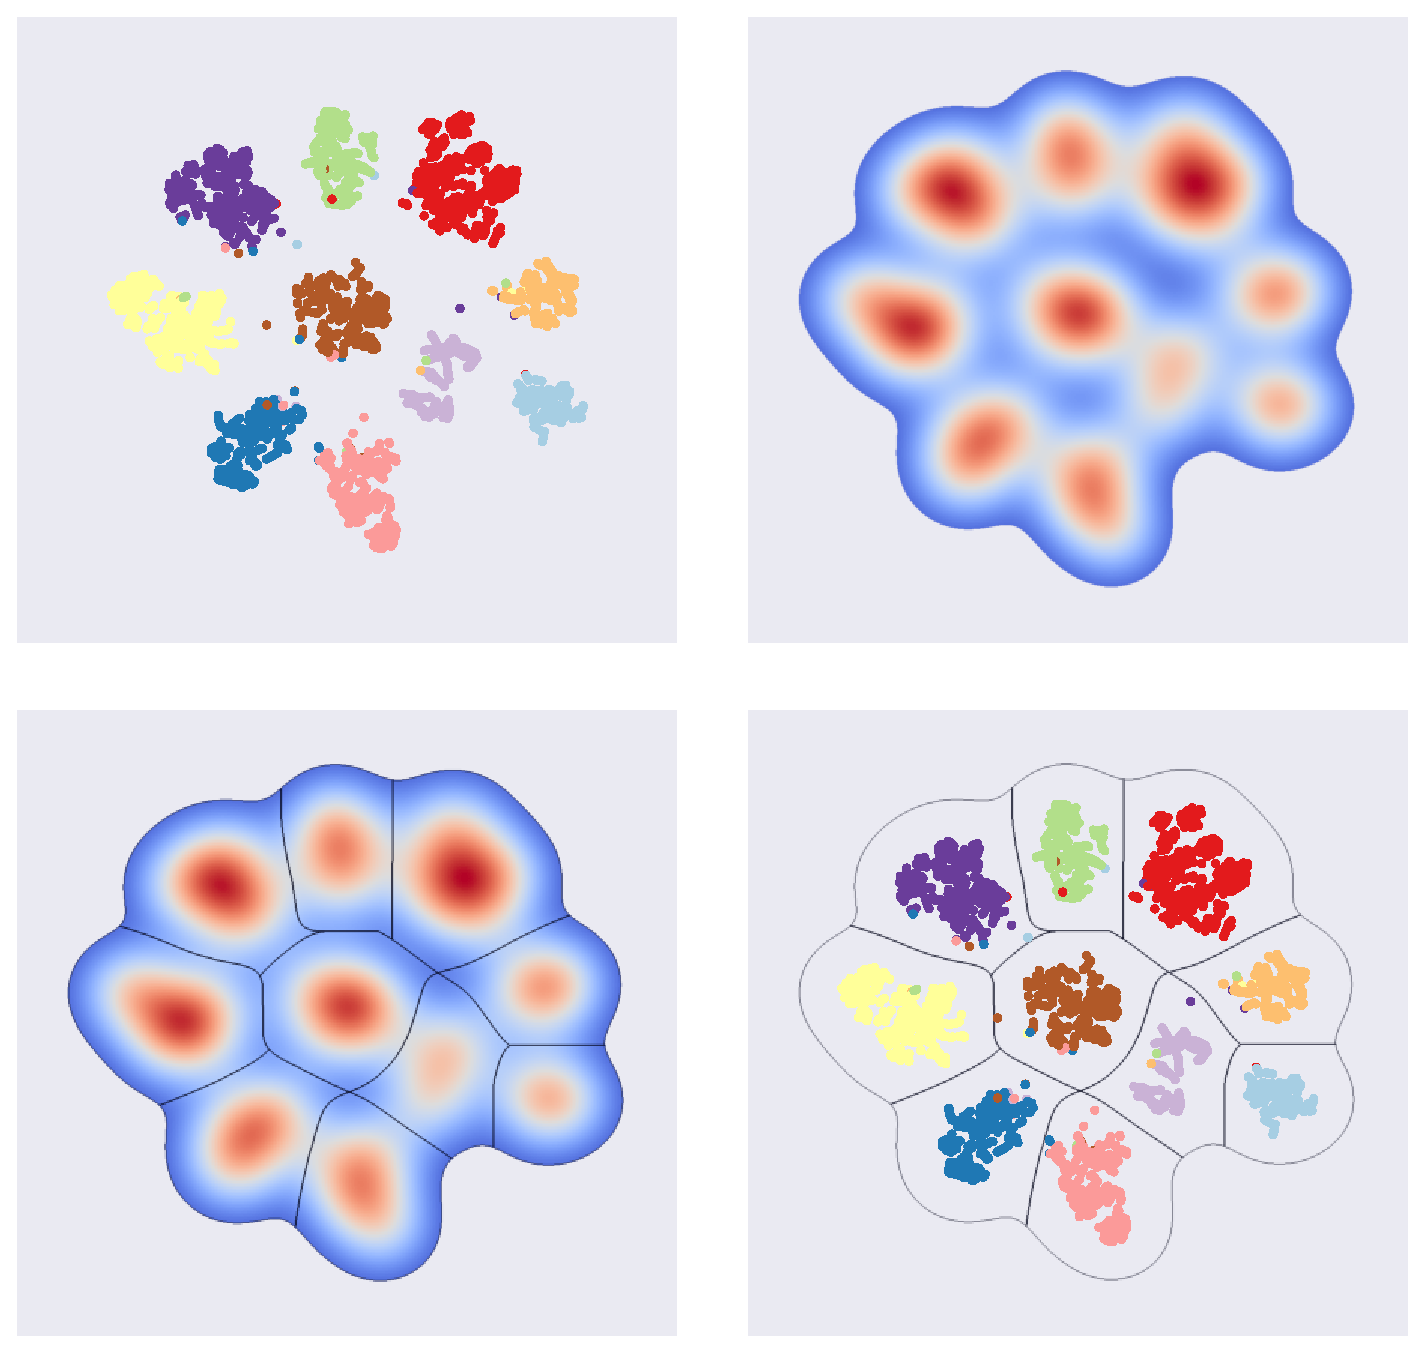
\includegraphics[width=0.8\linewidth]{./code/figures/clustering_example.pdf}
        \caption{Clustering the two-dimensional t-SNE embedding. \textit{Top left}: t-SNE embedding of simulated data, color coded by actual behavior. 
        \textit{Top right}: Kernel density estimation of the t-SNE embedding.
\textit{Bottom left}: Watershed segmentation applied to the kernel density estimation.
\textit{Bottom right}: Contours of the watershed segmentation with the t-SNE clusters shown inside.}
        \label{fig:clustering_example}
\end{figure}





\chapter{Methodology}
The starting point of the analysis is a set $\textbf{Y} =  \{ Y_d : d = 1, 2, \hdots, D \}$, where each set $Y_d$ is again a set of independent time series, $Y_d = \{ y_1^d(t), y_2^d(t), \hdots, y_n^d(t): t \in \{t_1, t_2, \hdots, t_{m_d} \} \}$.
Each $Y_d$ represents an animal for which $n$ time series are collected tracking parts of its movements.
Recording frequency is the same across animals.
The goal of the analysis is to cluster these time points into distinct distinguishable actions.

\textcolor{red}{Some summarization: "This is achieved by..."}

\section{Feature extraction}
\subsection{Detrending}
The first step is to analyse each time series separately, modifying them and thus creating $D \times n$ features which we will extract the behavioral information from.
Let $y_t = \{ y_1, y_2, \hdots, y_m \} = y_i^d(t)$ for some $d \in \{ 1, 2, \hdots, D \}$ and $i \in \{ 1, 2, \hdots, n \}$ be one such series.

\textcolor{red}{I don't see the point in centering the data around the mean before the detrending.}

We detrend the data as $y_t = s_3(t) + x_t$, $s_3(t)$ being the non-linear trend and $x_t$ the detrended time series.
The cubic spline $s_3(t)$ is found using least square regression as in equation \eqref{eq:lsq_spline} with equally spaced internal knots $\xi_1, \xi_2, \hdots, \xi_M$.
We choose the knots to have a fixed frequency, i.e., we choose $\Delta \xi= \xi_{i+1} - \xi_i, i = 2, \hdots, M$.
Figure \ref{fig:detrending_bc} shows an example of a detrended time series using cubic splines with interior knots every 240th time point.


\begin{figure}[tb ]
        \centering
        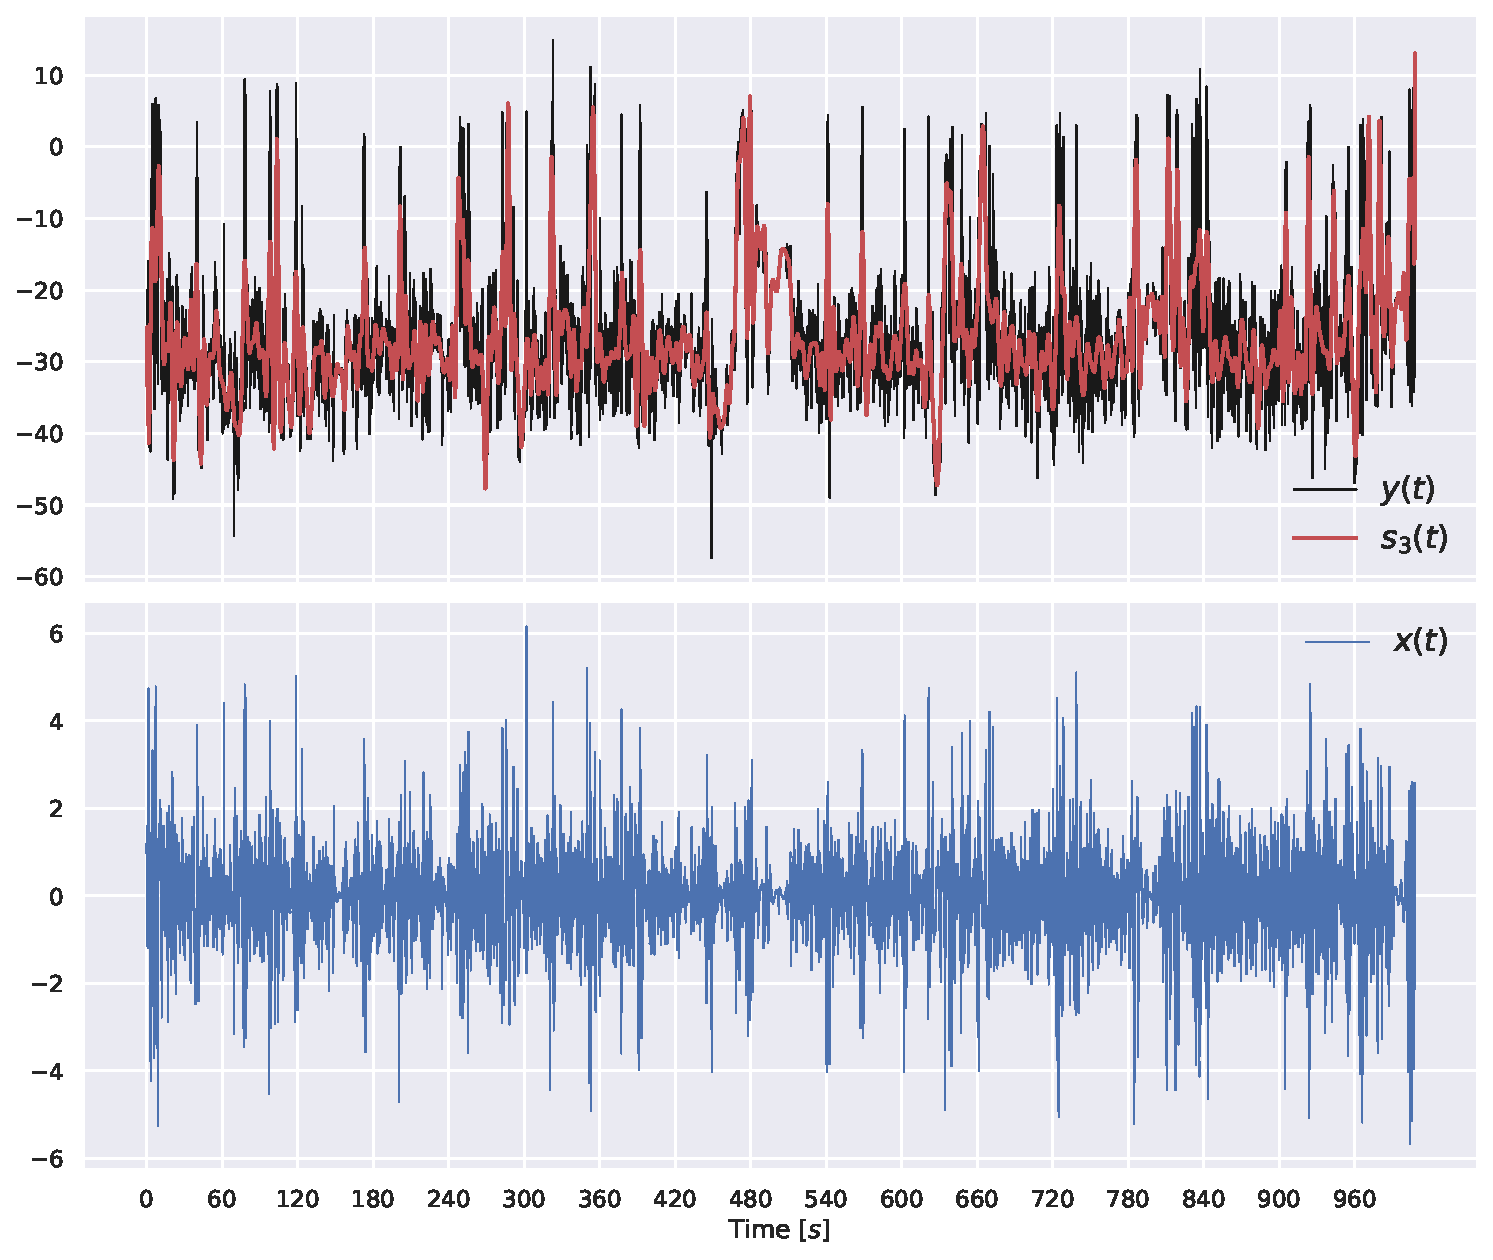
\includegraphics[width=\linewidth]{./code/figures/detrending/detrending_animal_1_BackPitch.pdf}
        \caption{Detrended time series using cubic spline regression.
        The top figure shows the original time series in black with the fitted trend in red.
The bottom figure shows the detrended time series.}
        \label{fig:detrending_bc}
\end{figure}


\subsection{Time frequency analysis}
To make the extracted features comparable, we normalize the time series by dividing it by its standard deviation
\begin{equation*}
        \sigma_x = \frac{1}{m}\sum_{t = 1}^{m} \left( x_t - \frac{1}{m}\sum_{i = 1}^{m}x_i \right)^2.
\end{equation*}
The detrended time series contain information about how the movements vary around the trend.
We assume this movement is repetitive in nature, and can be interpreted as a signal.
By applying time frequency analysis to the detrended time series, we obtain additional information about how the frequencies of these movements vary over time.
In turn this can contribute to detecting the behavioural clusters.

As we are unaware of at which scales these movements occur beforehand, we opt for a continuous wavelet transform as opposed to the short-time Fourier transform.
Let $J$ be the number of predefined frequency scales, ranging from $\omega_{\text{min}}$ to $\omega_{\text{max}}$.
The scales $s_1, s_2, \hdots, s_J$ in equation \eqref{eq:cwt_d} are chosen as fractional powers of two—as suggested in \cite{torrence}—e.g.,
\begin{align*}
        &s_j = \frac{2^{(j - 1)\delta j}}{\omega_{\text{max}}}, \quad j = 1, 2, \hdots, J, \\
        & \delta j = \frac{1}{J - 1} \log_2 \left( \frac{\omega_{\text{max}}}{\omega_{\text{min}}} \right).
\end{align*}
Choice of mother wavelet can for instance be based on expected features in the time series \cite{torrence}.
Using equation \eqref{eq:cwt_d} we compute the discrete continuous wavelet transform $\tilde{f}_m(s, \tau)$, and in turn the scaled scaleogram
\begin{equation}\label{eq:s_spec}
       \frac{1}{s_j} \left|\tilde{f}_m(s_j, t) \right|^2, \quad j = 1, 2, \hdots, J, \ t = 1, 2, \hdots, m.
\end{equation}
The scaling is done to keep the power comparable across the varying scales \cite{liu}.
An example plot of such a scaleogram is shown in figure \ref{fig:scaleogram_bc}.

\textcolor{red}{There is more done here, square root etc..}

\begin{figure}[tb]
        \centering
        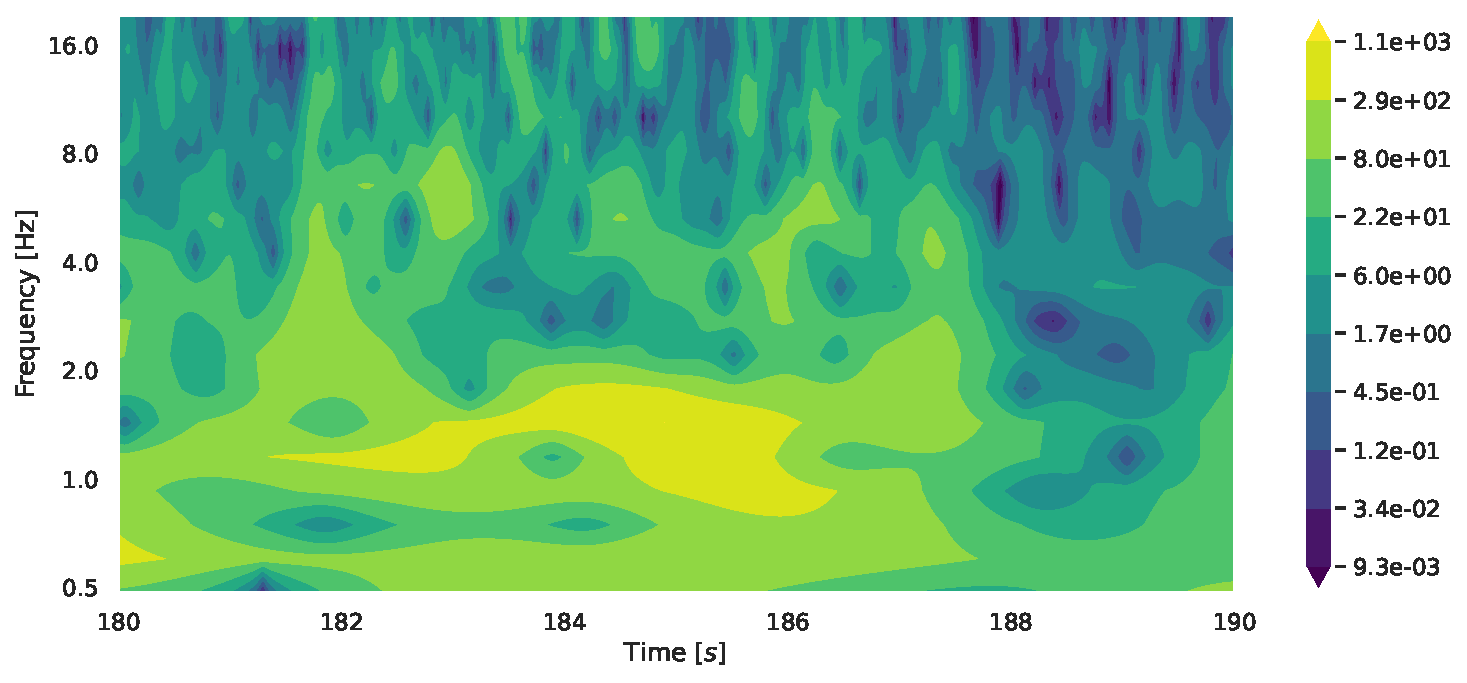
\includegraphics[width=\linewidth]{./code/figures/scaleograms/scaleogram_animal_1_BackPitch.pdf}
        \caption{Scaleogram of the continuous wavelet transform performed on the detrended time series shown in figure \ref{fig:detrending_bc}.
        The figure shows how the power at different frequency scales changes over time.}
        \label{fig:scaleogram_bc}
\end{figure}




\section{Manifold embedding}
After performing the time-frequency analysis on all time series for all animals, we concatenate the results into a new feature vector.
For animal $d$, we have $m_d$ time points, each containing information about the $n$ trend values, together with the $n \cdot J$ frequency powers.
The concatenated feature vector thus have dimension $(m_1 + m_2 + \hdots + m_D) \times (n \cdot (J + 1))$.
To cluster these time points into behaviours, we first reduce the feature dimension.
It is logical that there should exist strong correlations between the various frequencies.
\textcolor{red}{Insert discussion about why we do PCA first. Computation time for the t-SNE?}







\chapter{Discussion}
\section{Simulated Data}
To exemplify and visualize the impact of various implementation choices, we make use of simulated data inhibiting the properties we assume to be true for animal behaviour.
We simulate one animal with five recorded time series features, each over ten minutes with a recording frequency of 120Hz.
We create ten distinct behaviors.
For each behavior and feature, the underlying feature is generated as a superposition of four sine waves
\begin{equation*}
        \sum_{i = 1}^{4} a_i \sin (\omega_i 2 \pi t).
\end{equation*}
The $10 \times 5 \times 4$ frequencies $\omega$ are randomly generated uniformly between 0.5Hz and 20Hz.
Similarly, the amplitudes $a$ are randomly generated as a lognormal distribution with parameters $\mu_a = 1, \sigma_a = 0.5$.
A Gaussian noise is added with $\mu_n = 0, \sigma_n = 0.2$.
The length of the behaviors are modelled to follow an exponential distribution with mean $\lambda = 3$.
This is equivalent to generate $10 \cdot 60 / 3 = 200$ time points uniformly over $[0, 600]$, each interval assigned a random behavior.
Figure \ref{fig:color_coded_feature_1} shows one such feature, colored by the underlying behaviour at the first 50 seconds.


\begin{figure}[tb]
        \centering
        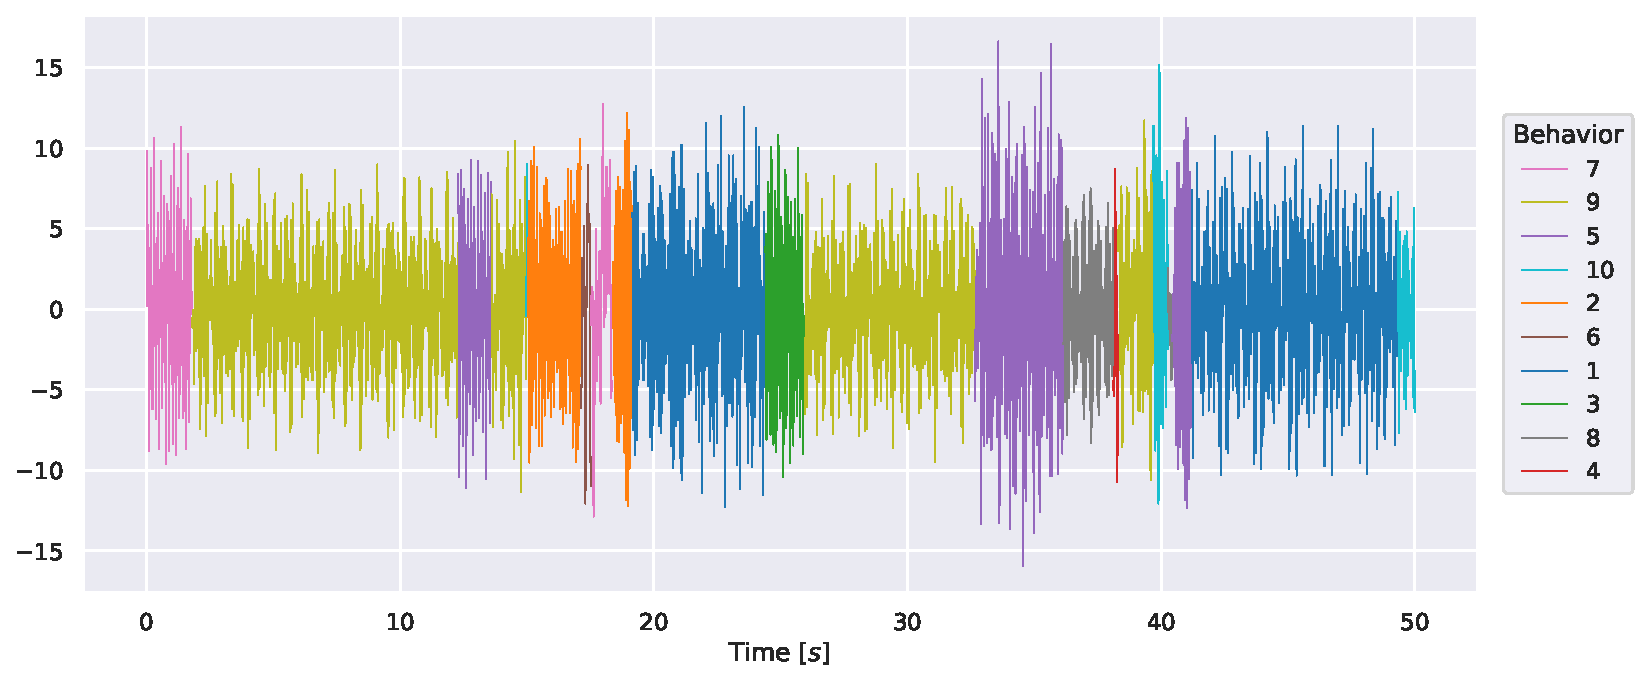
\includegraphics[width=1\linewidth]{./code/figures/simulated/features/color_coded_feature_1.pdf}
        \caption{Simulated feature vector showing changes in behavior during the first 50 seconds.}
        \label{fig:color_coded_feature_1}
\end{figure}


\section{Benefits of t-SNE}
There are many popular methods for embedding a high dimensional dataset into a lower dimensional space.
Principal component analysis is discussed in section \ref{sec:pca}, and is a good method to use for variance reduction.
It is also commonly used for visualizing data in two or three dimensions.
A large caveat is its linearity in the original features, which makes it unable to capture non-linear effects in the data.
Another common method is multidimensional scaling (MDS) \cite{hastie}.
It preserves the high dimensional distances as euclidean distances in the low dimensional space.
MDS emphasises the global structure in the data, as all points contribute significantly to the loss function.
There exists multiple methods extending the MDS methodology, making it more suitable for finding local and non-linear structures in the data. 
One of these methods is ISOMAP, which first creates a neighborhood graph, on which it computes geodesic distances between points as the shortest path in the graph \cite{tenenbaum}.
Using these distances it finds the low dimensional embedding via MDS.

As previously stated in section \ref{sec:tsne}, t-SNE preserves conditional probabilities created from the high dimensional euclidean distances \cite{hinton}.
Due to this it places emphasis on the local structure, and is a natural choice when the goal is to visualize high dimensional clusters in two dimensions.
Figure \ref{fig:dimensionality_reduction} illustrates these differences.
All methods are able to separate the clusters to some degree, bu t-SNE clearly stands out in its ability to distinguish them.

\begin{figure}[tb]
        \centering
        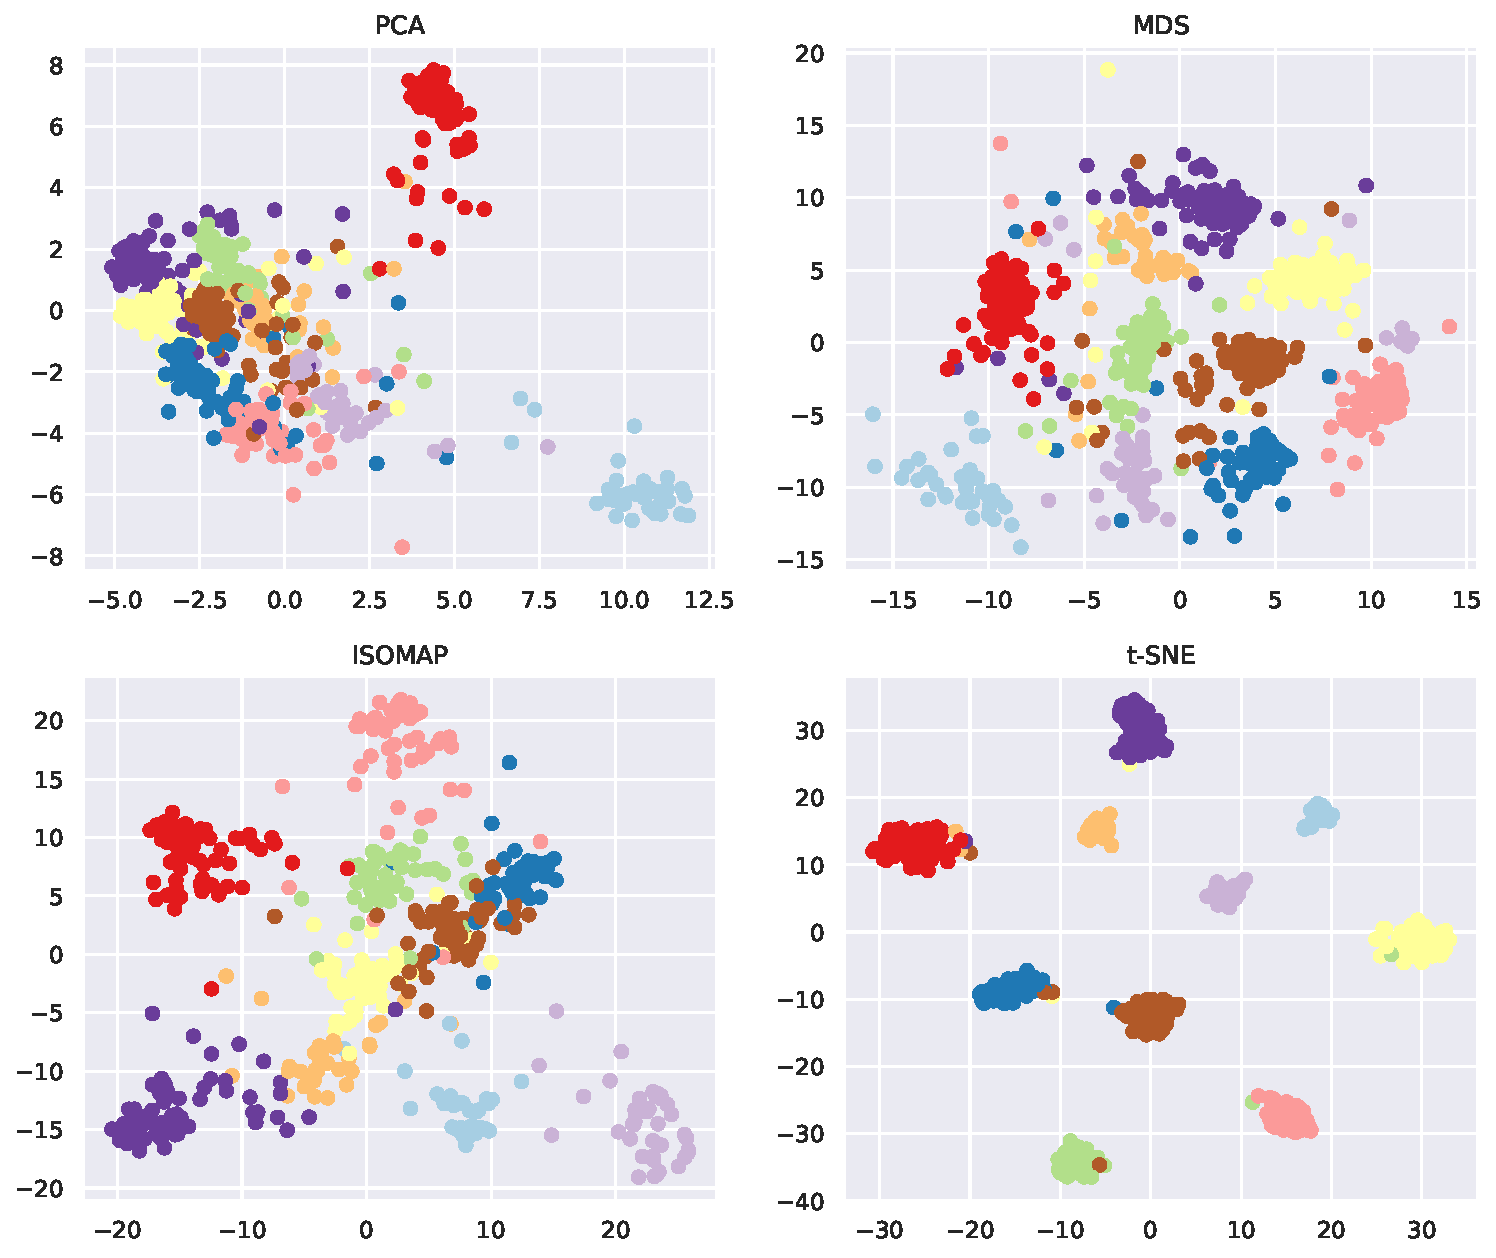
\includegraphics[width=1\linewidth]{./code/figures/dimensionality_reduction.pdf}
        \caption{Two dimensional embedding of the standardized simulated data using different dimensionality reduction methods.
        \textit{Top left:} Principal component analysis. 
\textit{Top right:} Multidimensional scaling.
\textit{Bottom left:} ISOMAP using $n = 20$ neighbors construction the graph.
\textit{Bottom right:} t-SNE with perplexity $30$.}
        \label{fig:dimensionality_reduction}
\end{figure}


\section{Tuning the perplexity parameter}
The perplexity parameter from equation \eqref{eq:perp} plays a significant role in the t-SNE embedding \cite{hinton}.
It is closely related to the number of neighbors considered when creating the conditional probabilities \eqref{eq:gaus}.
When the perplexity is small all points contribute "equally little" to the cost function, meaning the algorithm is not able to detect anything.
When the perplexity is large it attributes significance to more points, reducing the separation of clusters in the two dimensional embedding.
Large datasets should therefore need larges perplexity values.
Choosing it between 5 and 50 is suggested.
Figure \ref{fig:perplexity_tuning_simulated} shows how the perplexity parameter affects the clustering of the simulated data.
Perplexity values 30 and 50 give good results.
Note that only 3600 points were used calculating the embedding.


\begin{figure}[tb]
        \centering
        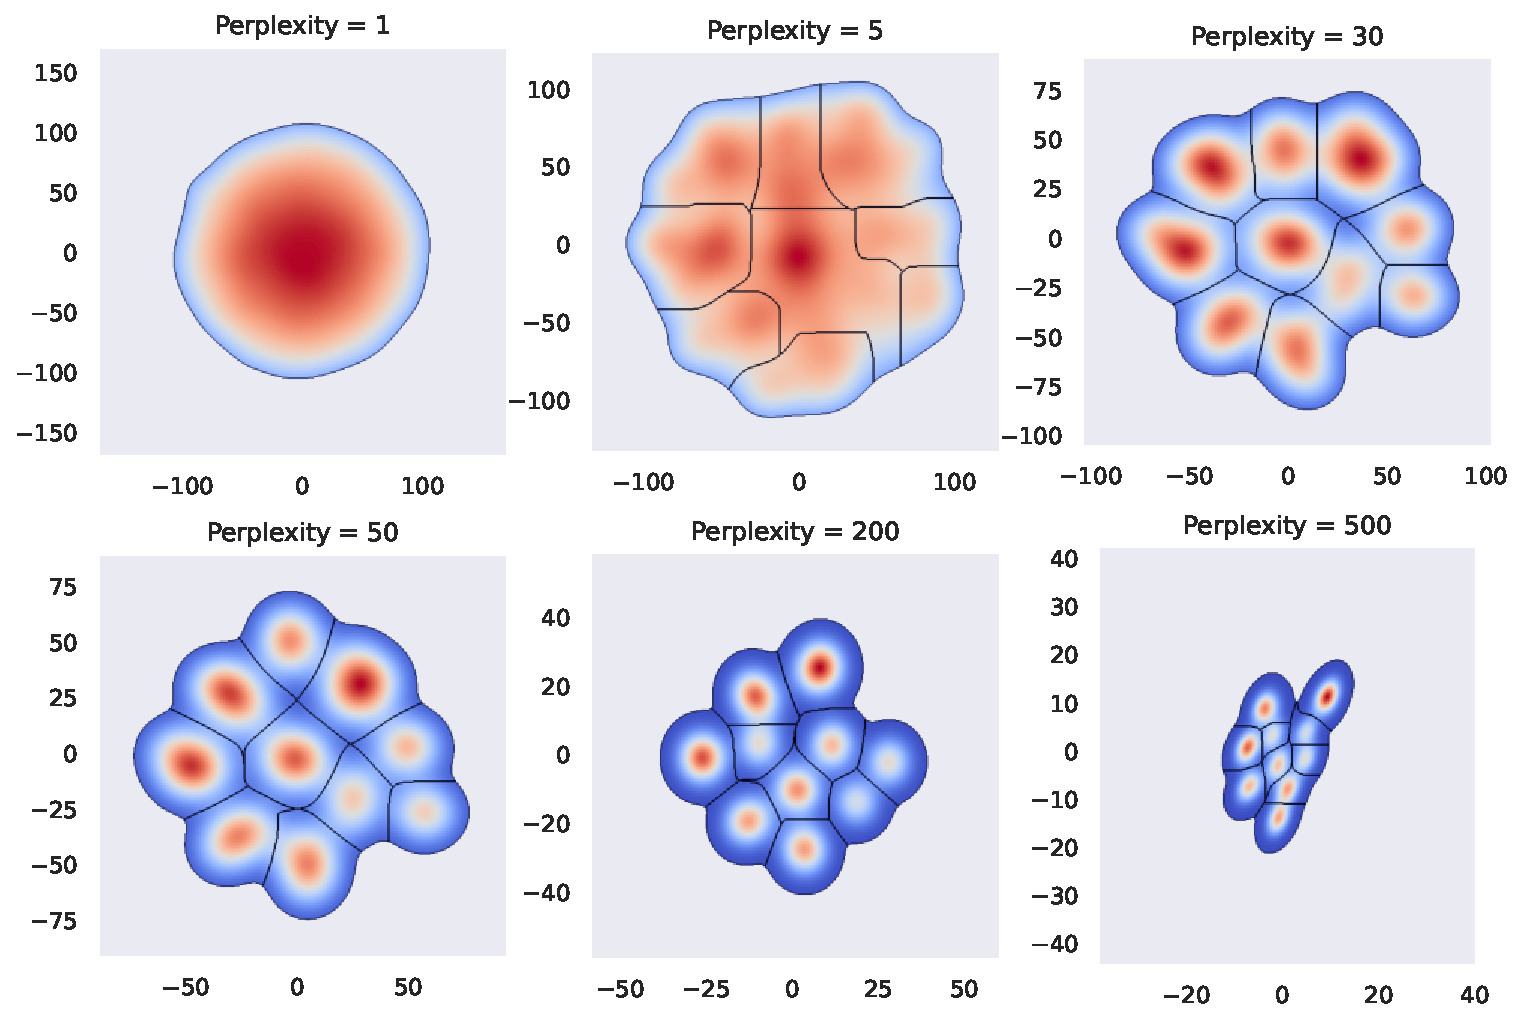
\includegraphics[width=1\linewidth]{./code/figures/perplexity_tuning_simulated.pdf}
        \caption{Clustering of the simulated data varying the perplexity parameter in t-SNE.
        The bandwidth for the kernel density estimation is 0.2 for all embeddings.}
        \label{fig:perplexity_tuning_simulated}
\end{figure}


\section{Pre embedding with PCA}
We could just embed the points directly into two dimensions through t-SNE alone.
However, due to memory complexity limitations in the t-SNE algorithm, we need to select a subset data points which we use to create the embedding.
These points can be thought of as the training points in the clustering algorithm.
How do we then classify the remaining data?
We will discuss two solutions to this problem.
Both solutions involves reducing the dimension of the data linearly through principal component analysis prior to the t-SNE embedding.
By only including the principal components explaining at least 95\% of the variance, we reduce a significant amount of noise.
At the same time we make it easier to compare data points through euclidean distances in the PCA space.

One idea is to apply kernel density estimation followed by watershed segmentation only on the training points.
I.e., we classify the training points first.
The remaining points are given the same label as their closest neighbor in the PCA space, using euclidean distance as the metric.

A second idea is to embed all points into the two dimensions provided by t-SNE on the training data. 
In this way, all points are contributing in the kernel density estimation, and subsequently in creating the behavioral regions.
This choice of direction has a significant impact on the resulting classification.
As shown in figure \ref{fig:pre_embed}.
\begin{figure}[tb]
        \centering
        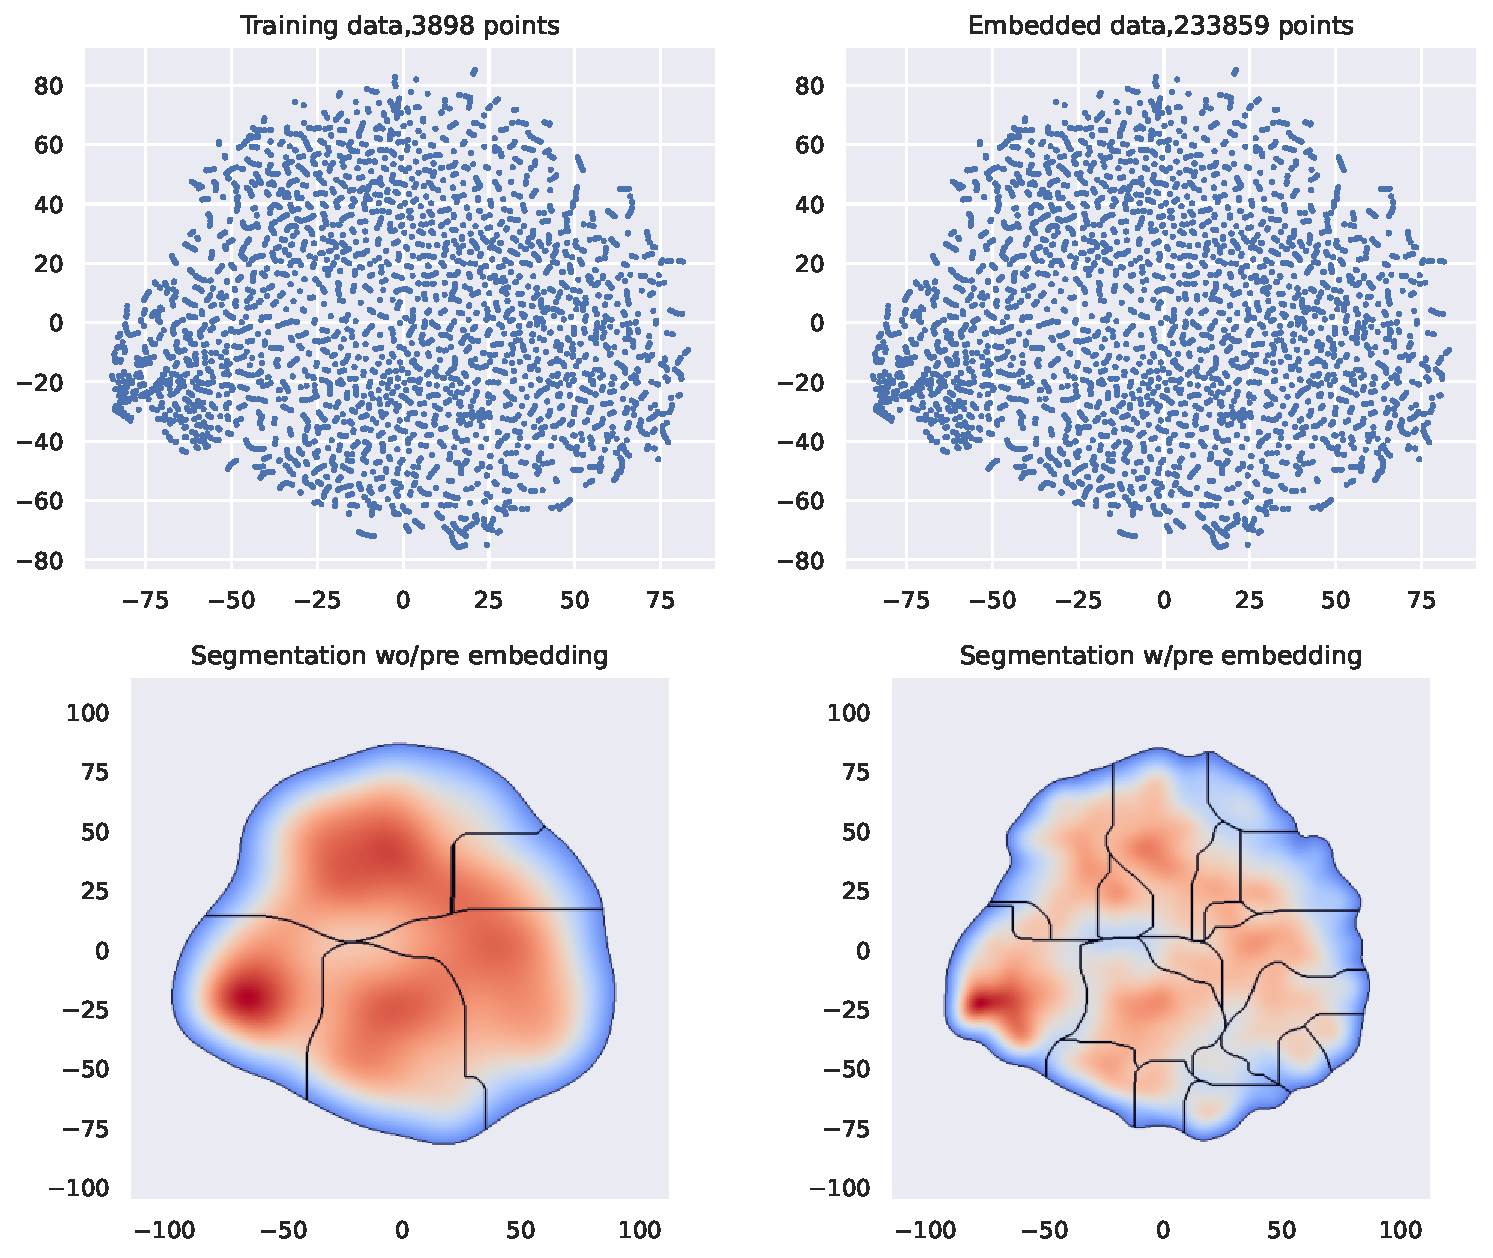
\includegraphics[width=1\linewidth]{./code/figures/test_pre_embed.pdf}
        \caption{}
        \label{fig:test_pre_embed}
\end{figure}

\section{Scaling the spectrogram}
It is the power spectrum provided by the wavelet transform which contains all the information we use to separate the behavioral clusters.
For each original feature we extract power at a range of frequencies, as shown in the scaleogram \ref{fig:scaleogram_bc}
As these are the features which is to be reduced into two dimensions, we need to prepare them as best as possible for the dimensionality reduction techniques.
Firstly we want all frequencies to contribute equally.
This creates the need for scaling across frequencies, as the wavelet transform creates larger spectral peaks for lower frequencies \cite{liu} \cite{berman}.
A suggested remedy for this is simply to divide the (squared) spectrum by its corresponding scale \cite{liu}.
Secondly all features should have equal contributions.
This is solved by standardizing the spectrum, which is commonly done before applying principal component analysis anyway.

Finally there remains the question of whether to take the square root of the wavelet spectrum, i.e, should we use $|\tilde{f}_n(s, \tau)|^2$ or $|\tilde{f}_n(s, \tau)|$ as a starting point for the dimensionality reduction.
Intuitively the squared spectrum discriminates more between frequencies with high and low power. 
When standardizing the power spectrum before PCA, the original magnitudes are unimportant.
However, without standardization taking the square root is essential in keeping the powers comparable, as shown in figure \ref{fig:test_scaling}.
The figure shows that standardizing groups the clusters more together in the t-SNE embedding, making it harder to distinguish very dissimilar clusters.
\begin{figure}[tb]
        \centering
        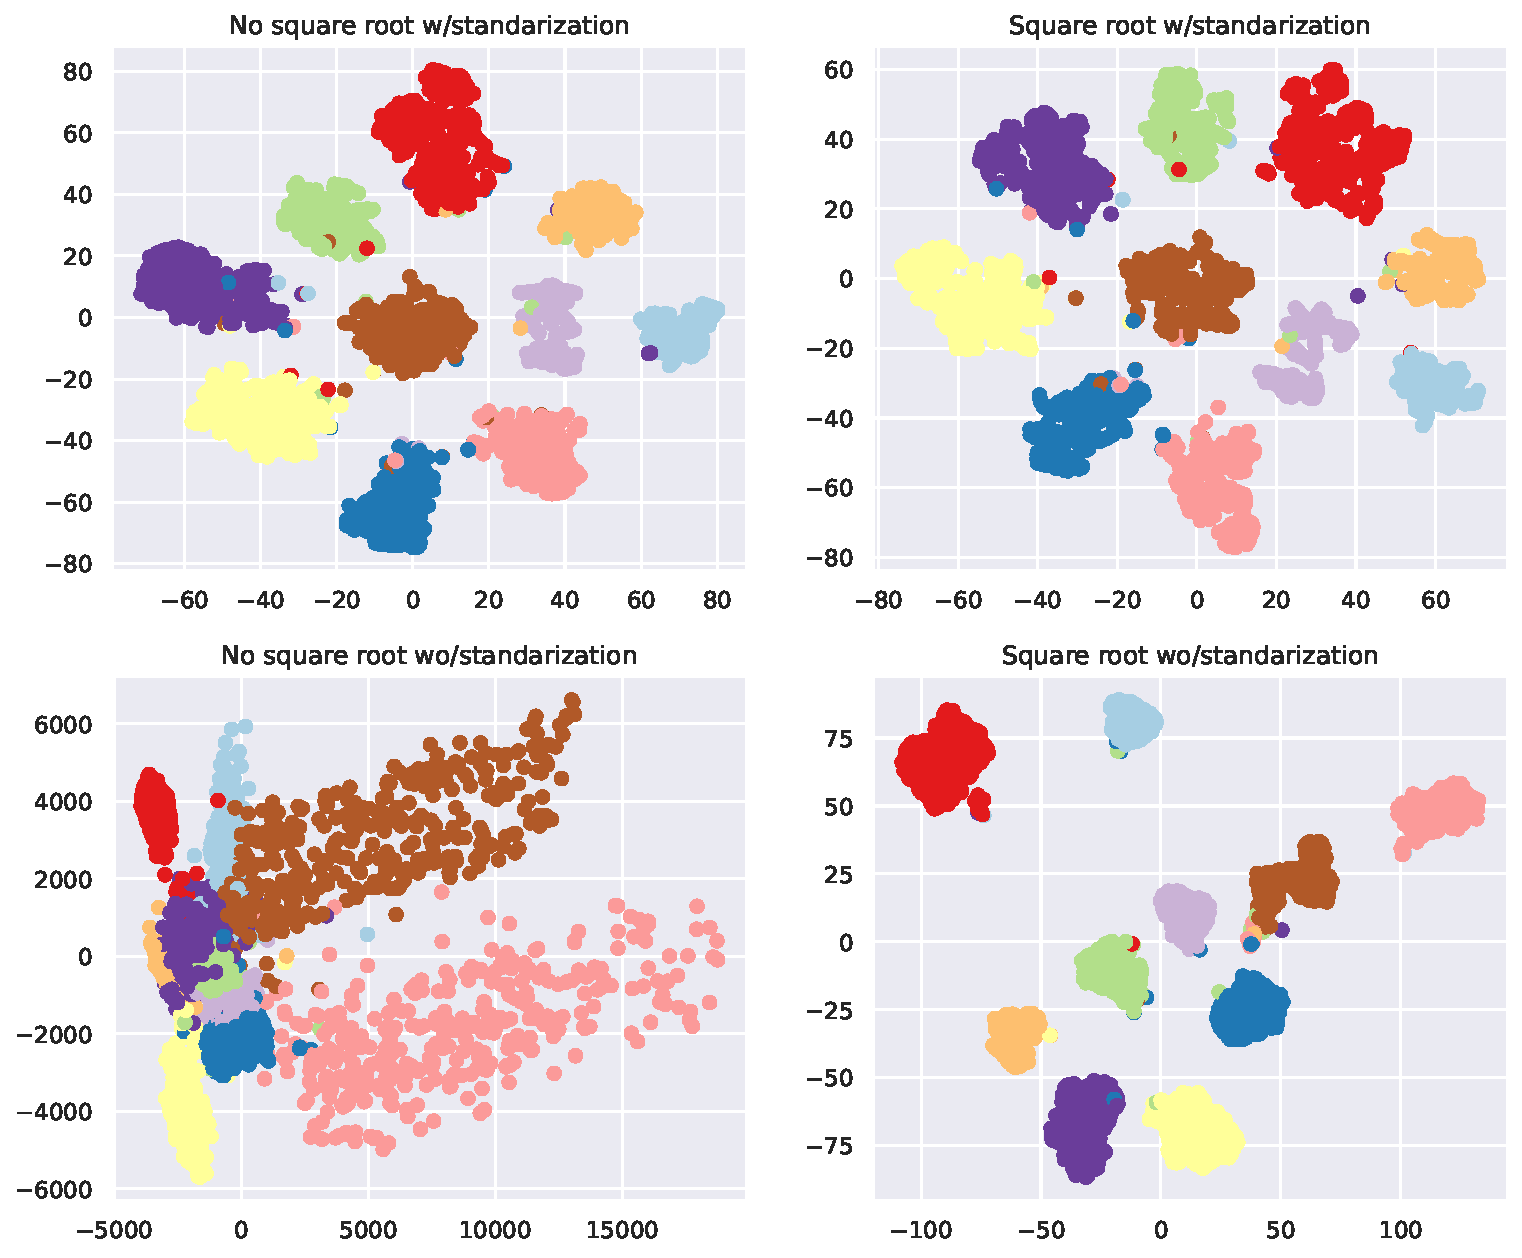
\includegraphics[width=1\linewidth]{./code/figures/test_scaling.pdf}
        \caption{t-SNE embedding of the simulated data varying the scaling of the wavelet power spectrum.
        Points are color coded by their underlying true behavior.}
        \label{fig:test_scaling}
\end{figure}

When tested on actual data, figure \ref{fig:test_scaling_example} shows that omitting the standardization creates several outliers in the t-SNE embedding, without providing clearer separation of clusters.
\begin{figure}[tb]
        \centering
        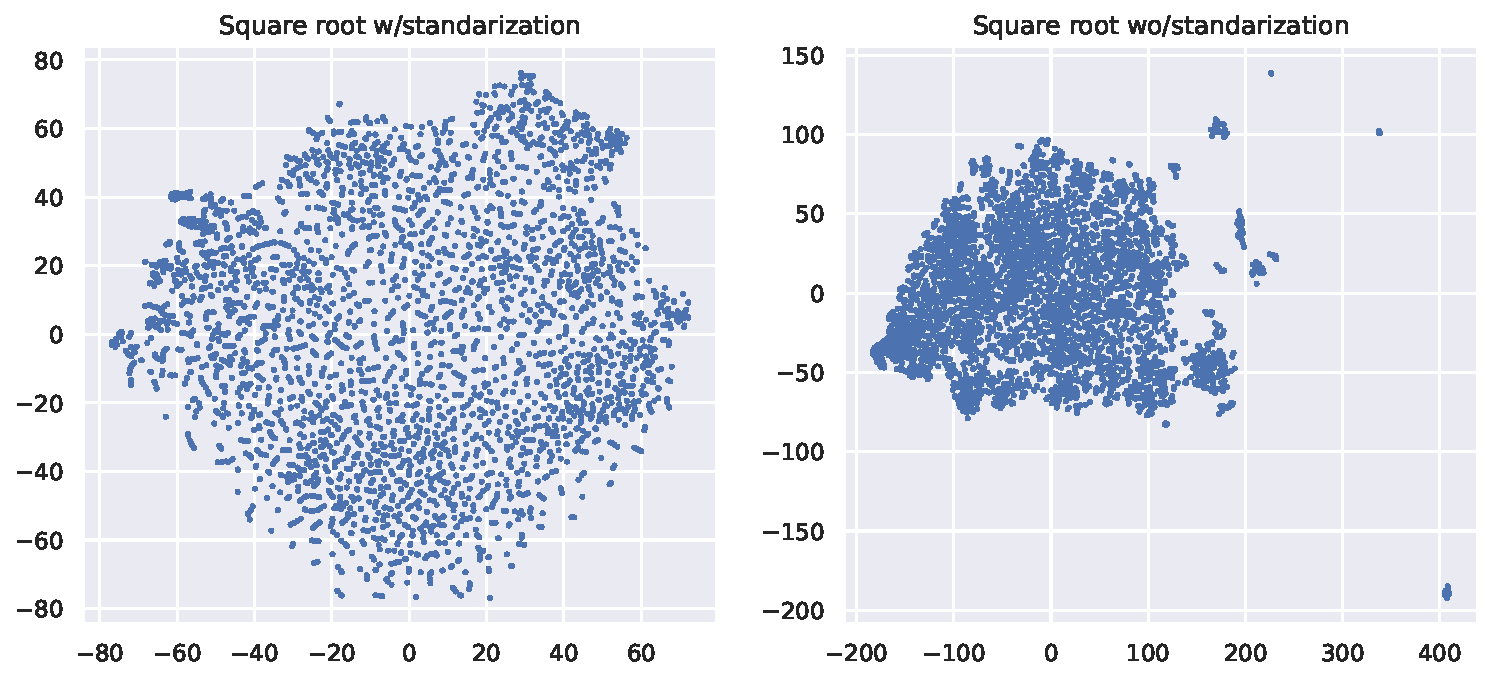
\includegraphics[width=1\linewidth]{./code/figures/test_scaling_example.pdf}
        \caption{t-SNE embedding of motion recordings of two rats downsampled at 2Hz.
        On the left the wavelet spectrum is standardized before applying PCA.
On the right no standardization is performed.}
        \label{fig:test_scaling_example}
\end{figure}


\section{Effects of downsampling}


\section{Tuning the bandwidth matrix}
The kernel density estimation \eqref{eq:kde} plays a significant role in final the clustering.
It smooths the two dimensional embedding creating local peaks which we interpret as individual behaviors.
The degree of smoothing is determined by the bandwidth $2 \times 2$ matrix $H$ briefly discussed in section \ref{sec:kde}.
Several ways of choosing this parameter have been discussed in literature, most of them based on minimizing the asymptotic mean integrated squared error \cite{simonoff}.
As our goal is visualizing clusters, it is better to test several different values, choosing the one which provide the best visualization.
To limit the possibilities, we let the scaling be identical in both dimensions, letting $H$ be a diagonal matrix with identical elements.





\chapter{Results}
\textcolor{red}{
\begin{itemize}
        \item Present the actual data, and the resulting embedding and some notes on the results if time permits
\end{itemize}}


\chapter{Conclusions}
\textcolor{red}{
\begin{itemize}
        \item Does it work?
        \item How do we know the model is good?
        \item What further testing is required?
\end{itemize}}



\newpage
\printbibliography
\end{document}



